\documentclass[12pt]{article}
%
\usepackage{graphicx}
\usepackage[margin=1in,footskip=0.2in]{geometry}%big footskip brings number down, smal
\usepackage{amsmath}
\usepackage{amssymb}
\usepackage[T1]{fontenc}
\usepackage{listings}
\usepackage{bm}
\usepackage{hyperref}
\usepackage{setspace}
\usepackage[usenames]{color}
\usepackage[utf8]{inputenc}
\usepackage{psfrag}
\usepackage[table,xcdraw]{xcolor}
\usepackage{pdflscape}
\usepackage{tikz}
\usepackage{csvsimple}

%\usepackage{titlesec}
%\usepackage[percent]{overpic}
%\usepackage{wrapfig}
%\usepackage{relsize}
%\usepackage{dsfont}

%\setcounter{secnumdepth}{4}

%\titleformat{\paragraph}
%{\normalfont\normalsize\bfseries}{\theparagraph}{1em}{}
%\titlespacing*{\paragraph}
%{0pt}{3.25ex plus 1ex minus .2ex}{1.5ex plus .2ex}

%
\begin{document}

%%
%\title{Short-Term Panel Requests: Improving Catch Estimation Methods in Sparsely Sampled Mixed-Stock Fisheries.}
%\author{Nick Grunloh$^\text{a}$, Edward Dick$^\text{b}$, Don Pearson$^\text{b}$, Marc Mangel$^\text{a,c}$, John Field$^\text{b}$}
%\date{\today}
%\maketitle
%\noindent
%$^\text{a}$ Center for Stock Assessment Research, University of California, Santa Cruz, Mail Stop SOE-2, Santa Cruz, CA 95064, USA.\\
%$^\text{b}$ Fisheries Ecology Division, Southwest Fisheries Science Center, National Marine Fisheries Service, National Oceanographic and Atmospheric Administration, 110 McAllister Way, Santa Cruz, CA 95060, USA.\\
%$^\text{c}$ Department of Applied Mathematics and Statistics, Jack Baskin School of Engineering, University of California, Santa Cruz, Mail Stop SOE-2, Santa Cruz, CA 95064, USA.

%
\clearpage
%
\section{Diagnostic template and full predictive performance}


%\includegraphics[width=\textwidth]{https://github.com/gasduster99/sppComp/blob/master/try1/postSSC/95619831990M3.5/sppMad68.pdf}

\href{https://github.com/gasduster99/sppComp/blob/master/try1/postSSC/95619831990M3.5/sppMad68.pdf}{link test}

\begin{itemize}
	\item describe general predictive perfomance plot (show single page 68 and 95 example)
	\item describe MAD metric (show equation)
	\item show MAD picture
	\item describe how to use it to find poor performing stratum
	\item show marginal diagnostic
	\item show spp-year-gear and spp-year diagnostics
	\item describe and link full diagnostic csv
\end{itemize}

%
\clearpage
%
\section{Time model and prior sensitivities}

\subsection{MCAT 250 Time Models}	
	\begin{table}[ht!]
	\centering
	\begin{tabular}[c]{@{}lcccccc@{}}
	%\toprule
	\hline
	& M1 & M2 & M3 & M4 & M5 & M6 \\ \hline
	\(\Delta\) DIC & 6448.98 & 0.33 & 0 & 4.45 & 9.3 & 7.42 \\
	\(\Delta\) WAIC & 6421.5 & 0.37 & 0 & 4.52 & 8.25 & 6.55 \\
	\(pr(M|y)\) & 0 & 0 & 0 & 0.03 & 0 & 0.97
	\end{tabular}
	\end{table}

\subsubsection{\href{https://github.com/gasduster99/sppComp/tree/master/sscRuns/25019781982M3}{M3}, \href{https://github.com/gasduster99/sppComp/tree/master/sscRuns/25019781982M4}{M4}, \href{https://github.com/gasduster99/sppComp/tree/master/sscRuns/25019781982M6}{M6} \href{https://github.com/gasduster99/sppComp/tree/master/try1/postSSC/25019781982M3M4M6}{Comparision}}
	\begin{figure}[ht!]
	\centering
	\includegraphics[width=.6\textwidth]{../sscRuns/25019781982M3/sppMad68.pdf}
	\end{figure}

	\begin{figure}[ht!]
        \centering
        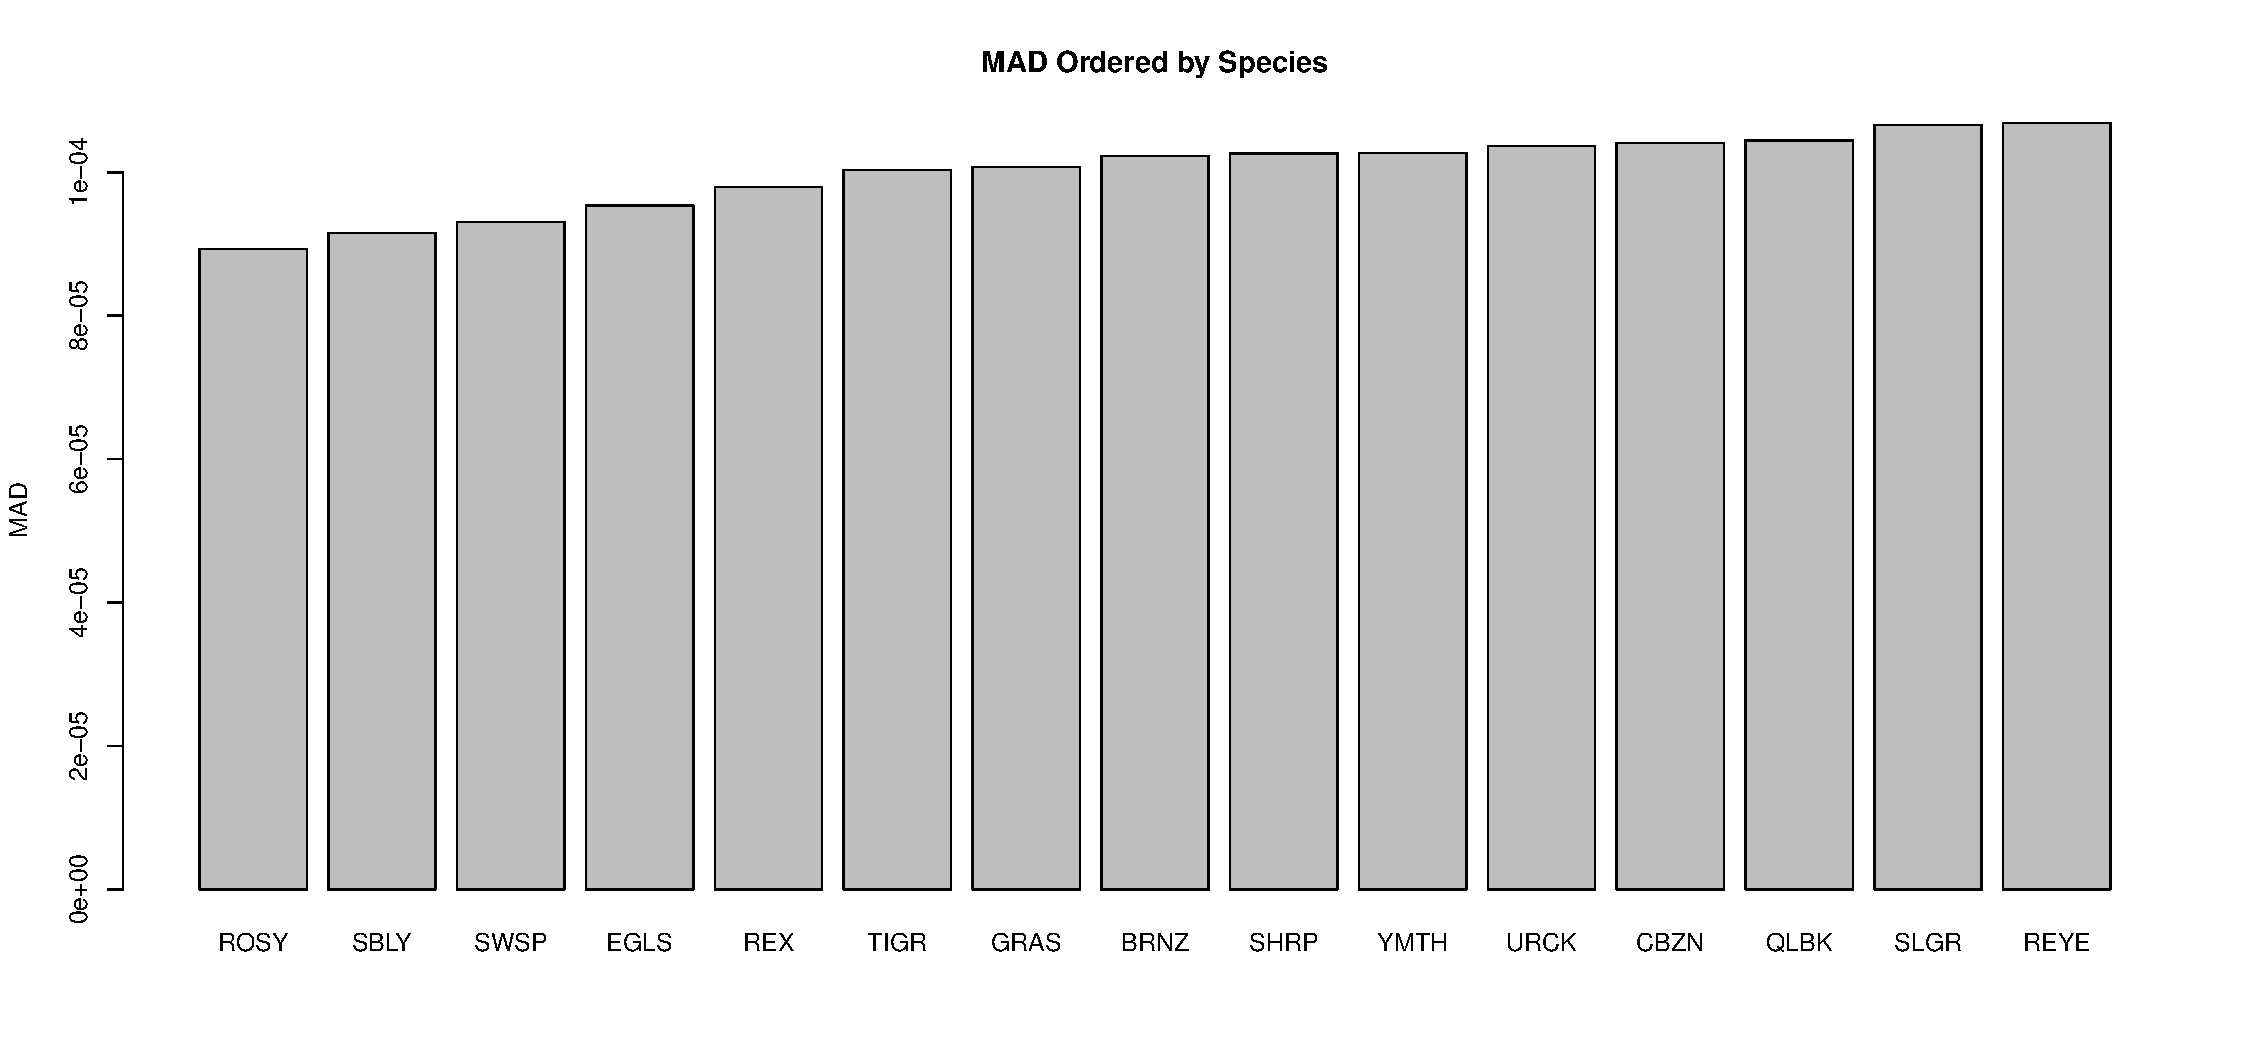
\includegraphics[width=.6\textwidth]{../sscRuns/25019781982M4/sppMad68.pdf}
        \end{figure}
	
	\begin{figure}[ht!]
        \centering
        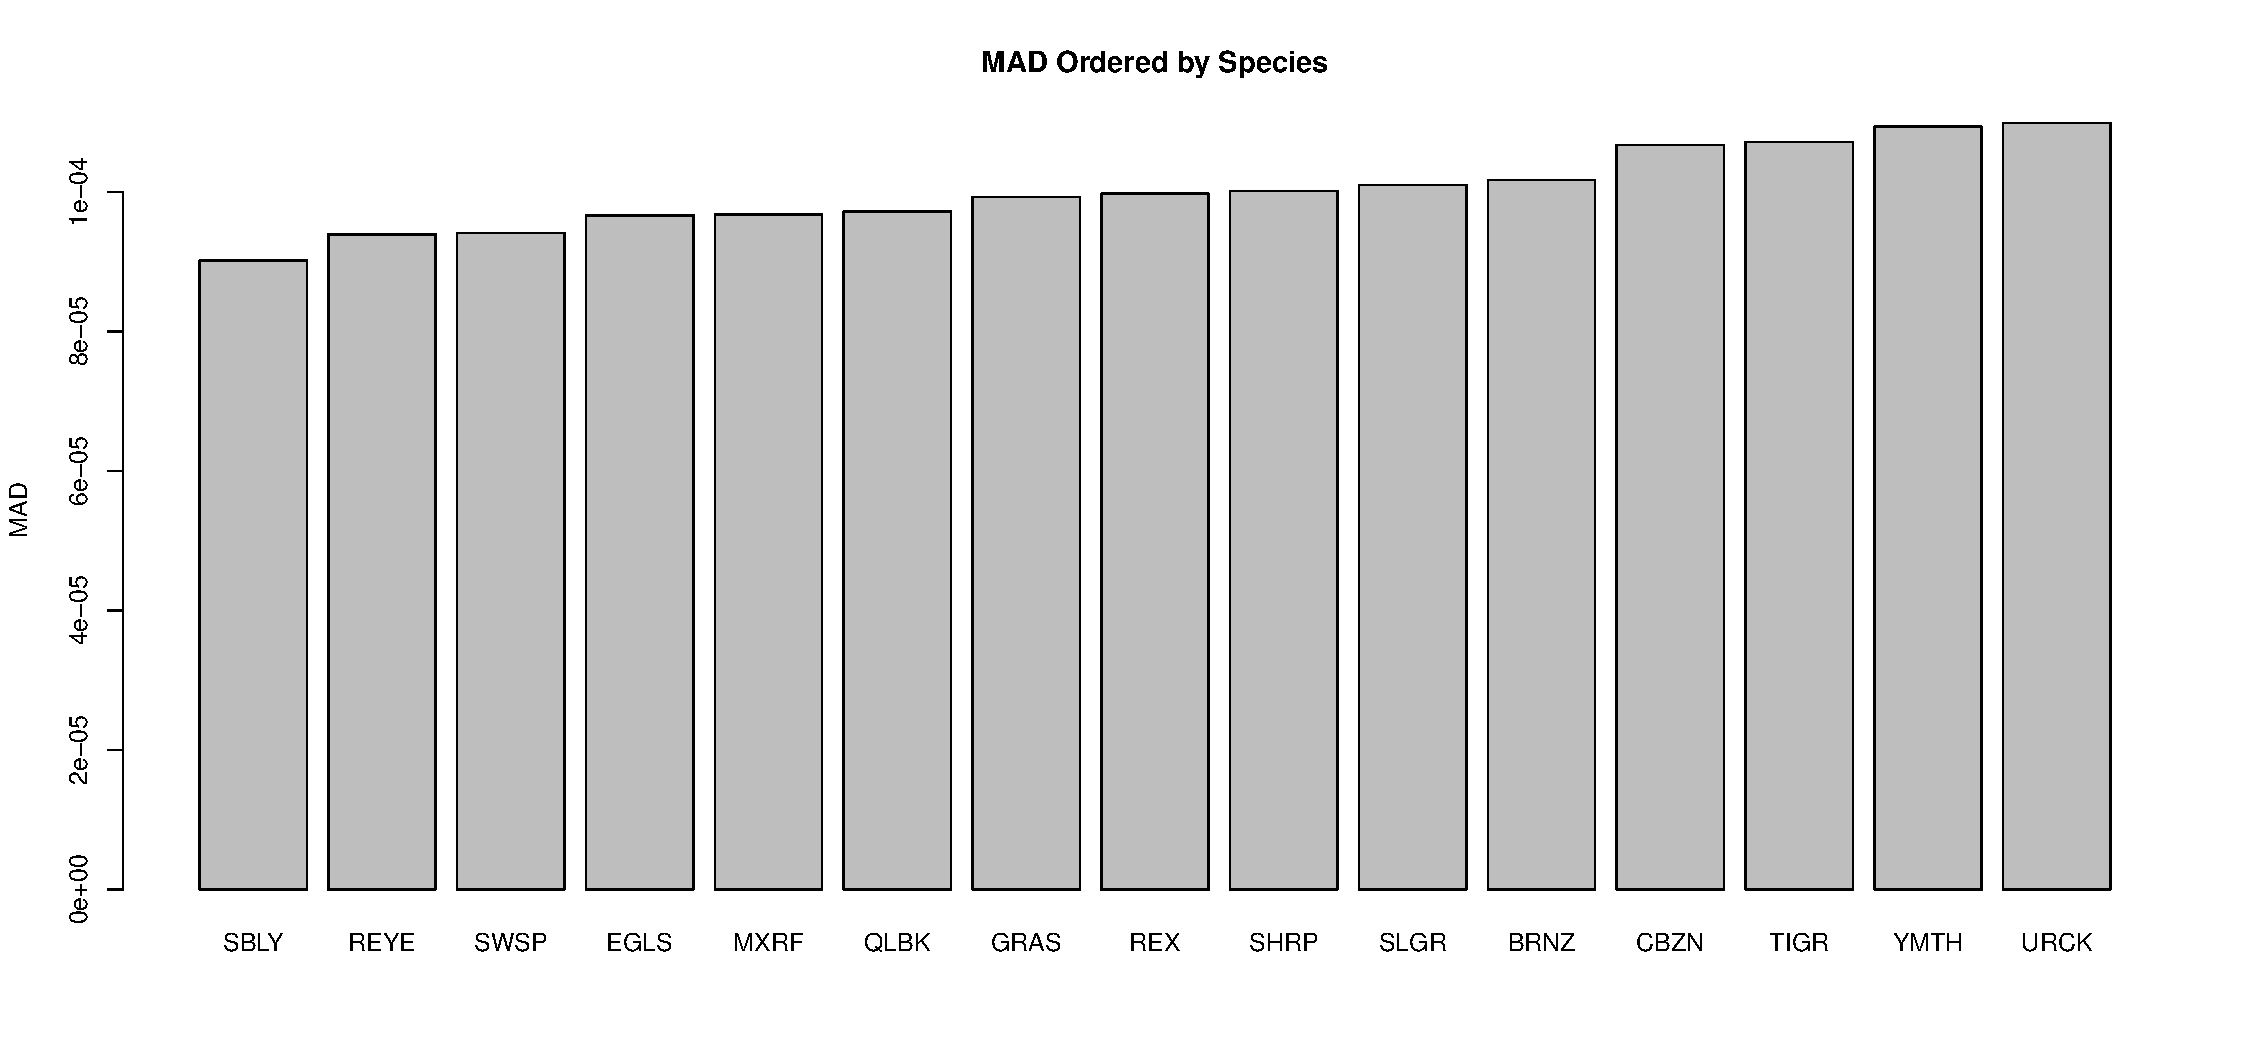
\includegraphics[width=.6\textwidth]{../sscRuns/25019781982M6/sppMad68.pdf}
        \end{figure}
	
	\clearpage
	\begin{figure}[ht!]
        \centering
        \includegraphics[width=1.1\textwidth]{{./postSSC/25019781982M3M4M6/marginalBCAC/marginalBCAC-0.68-Diagnostic}.pdf}
        \end{figure}

	\clearpage
	\begin{figure}[ht!]
        \centering
        \includegraphics[width=1.1\textwidth]{{./postSSC/25019781982M3M4M6/marginalWDOW/marginalWDOW-0.68-Diagnostic}.pdf}
        \end{figure}

	\clearpage
	\begin{figure}[ht!]
        \centering
        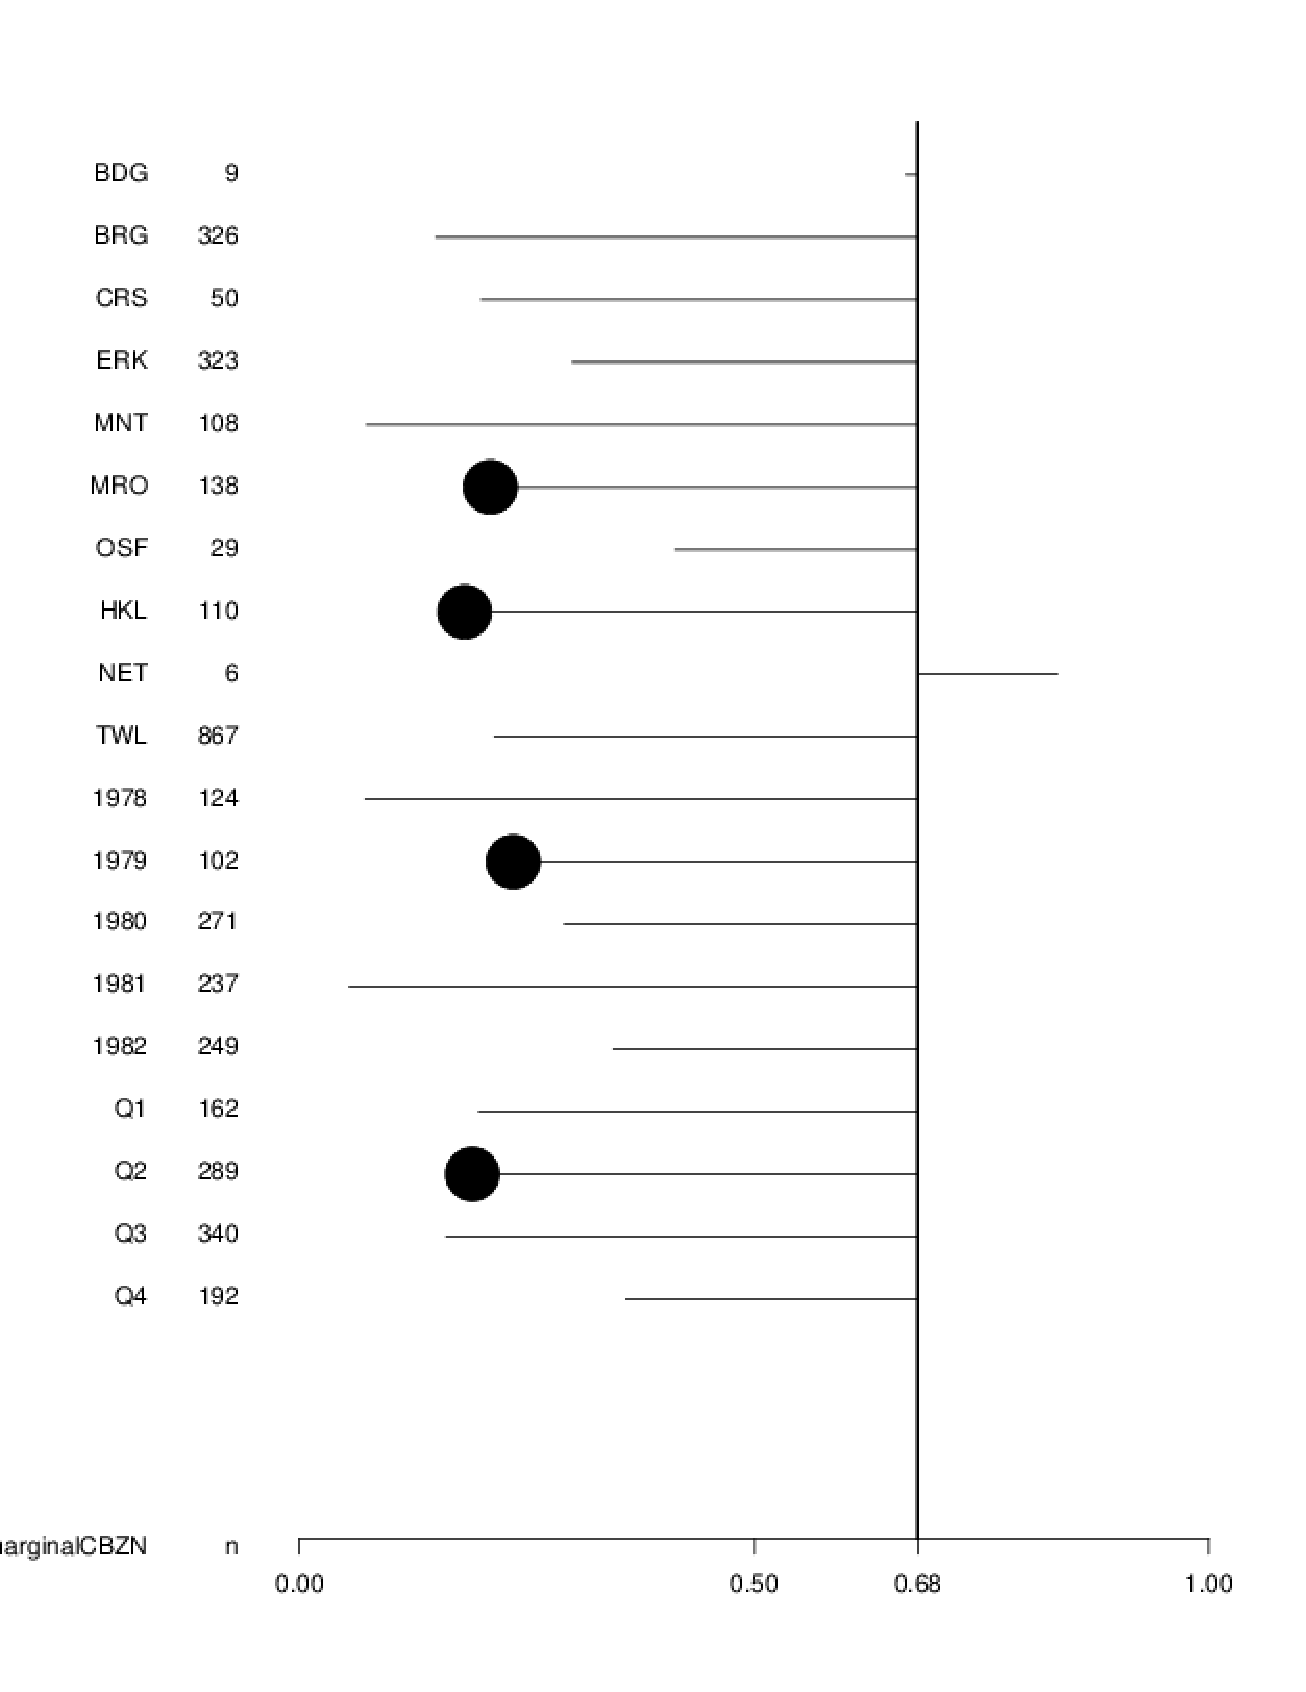
\includegraphics[width=1.1\textwidth]{{./postSSC/25019781982M3M4M6/marginalCBZN/marginalCBZN-0.68-Diagnostic}.pdf}
        \end{figure}
	
	\clearpage
	\begin{figure}[ht!]
        \centering
        \includegraphics[width=1.1\textwidth]{{./postSSC/25019781982M3M4M6/marginalURCK/marginalURCK-0.68-Diagnostic}.pdf}
        \end{figure}


%\clearpage
%\subsubsection{M3}
%	\begin{figure}[ht!]
%	\centering
%	\includegraphics[width=1\textwidth]{../sscRuns/25019781982M3/sppMad68.pdf}
%	\end{figure}
%
%	\begin{figure}[ht!]
%	\centering
%	\includegraphics[width=1.1\textwidth]{{../sscRuns/25019781982M3/marginalRDBD/marginalRDBD-0.68-Diagnostic}.pdf}
%	\end{figure}
%
%	\begin{figure}[ht!]
%	\centering
%	\includegraphics[width=1.1\textwidth]{{../sscRuns/25019781982M3/marginalWDOW/marginalWDOW-0.68-Diagnostic}.pdf}
%	\end{figure}	
%	
%	\begin{figure}[ht!]
%	\centering
%	\includegraphics[width=1.1\textwidth]{{../sscRuns/25019781982M3/marginalBRNZ/marginalBRNZ-0.68-Diagnostic}.pdf}
%	\end{figure}
%
%	\begin{figure}[ht!]
%	\centering
%	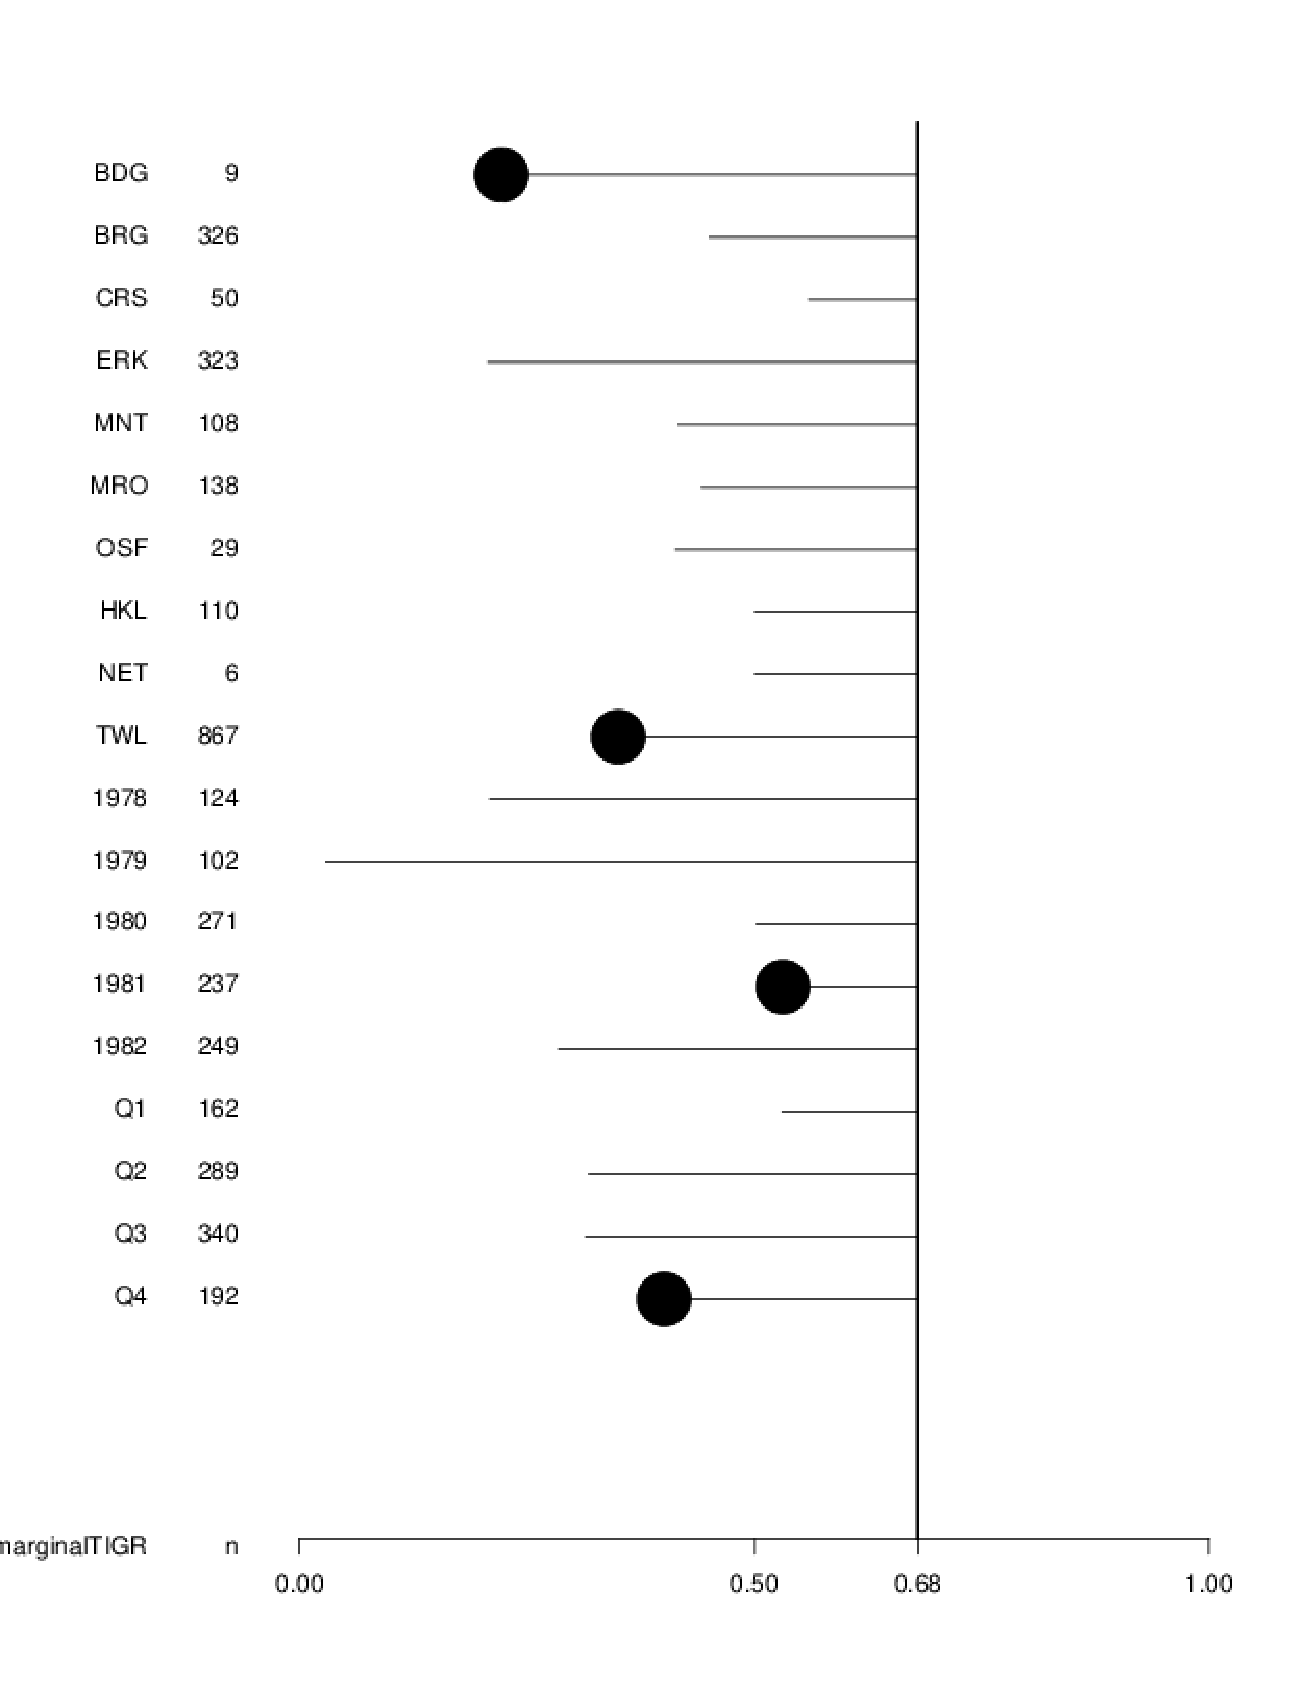
\includegraphics[width=1.1\textwidth]{{../sscRuns/25019781982M3/marginalTIGR/marginalTIGR-0.68-Diagnostic}.pdf}
%	\end{figure}
%	
%	%\begin{figure}[ht!]
%	%\centering
%	%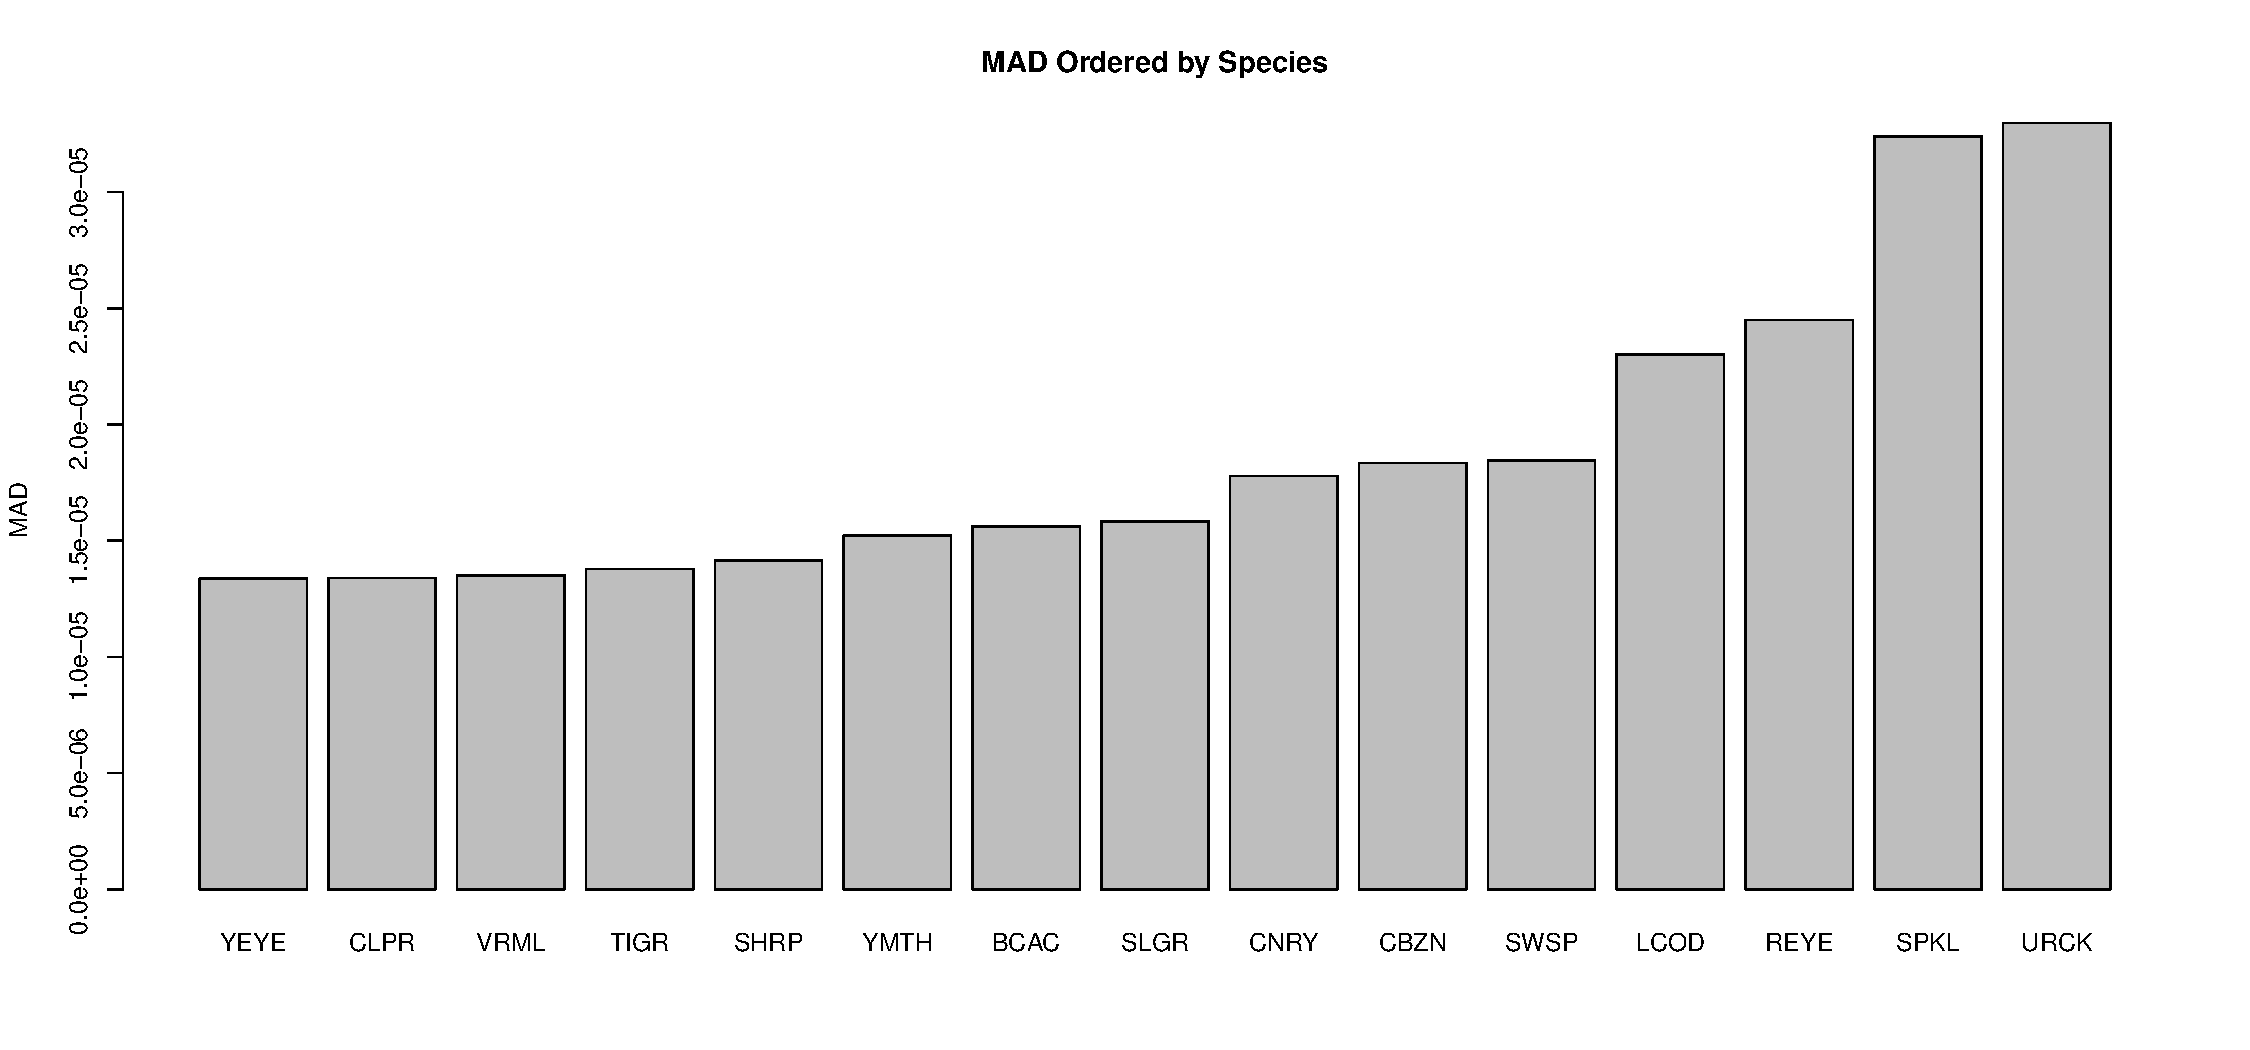
\includegraphics[width=1.1\textwidth]{../sscRuns/25019781982M3/sppMad95.pdf}
%	%\end{figure}
%	%
%	%\begin{figure}[ht!]
%	%\centering
%	%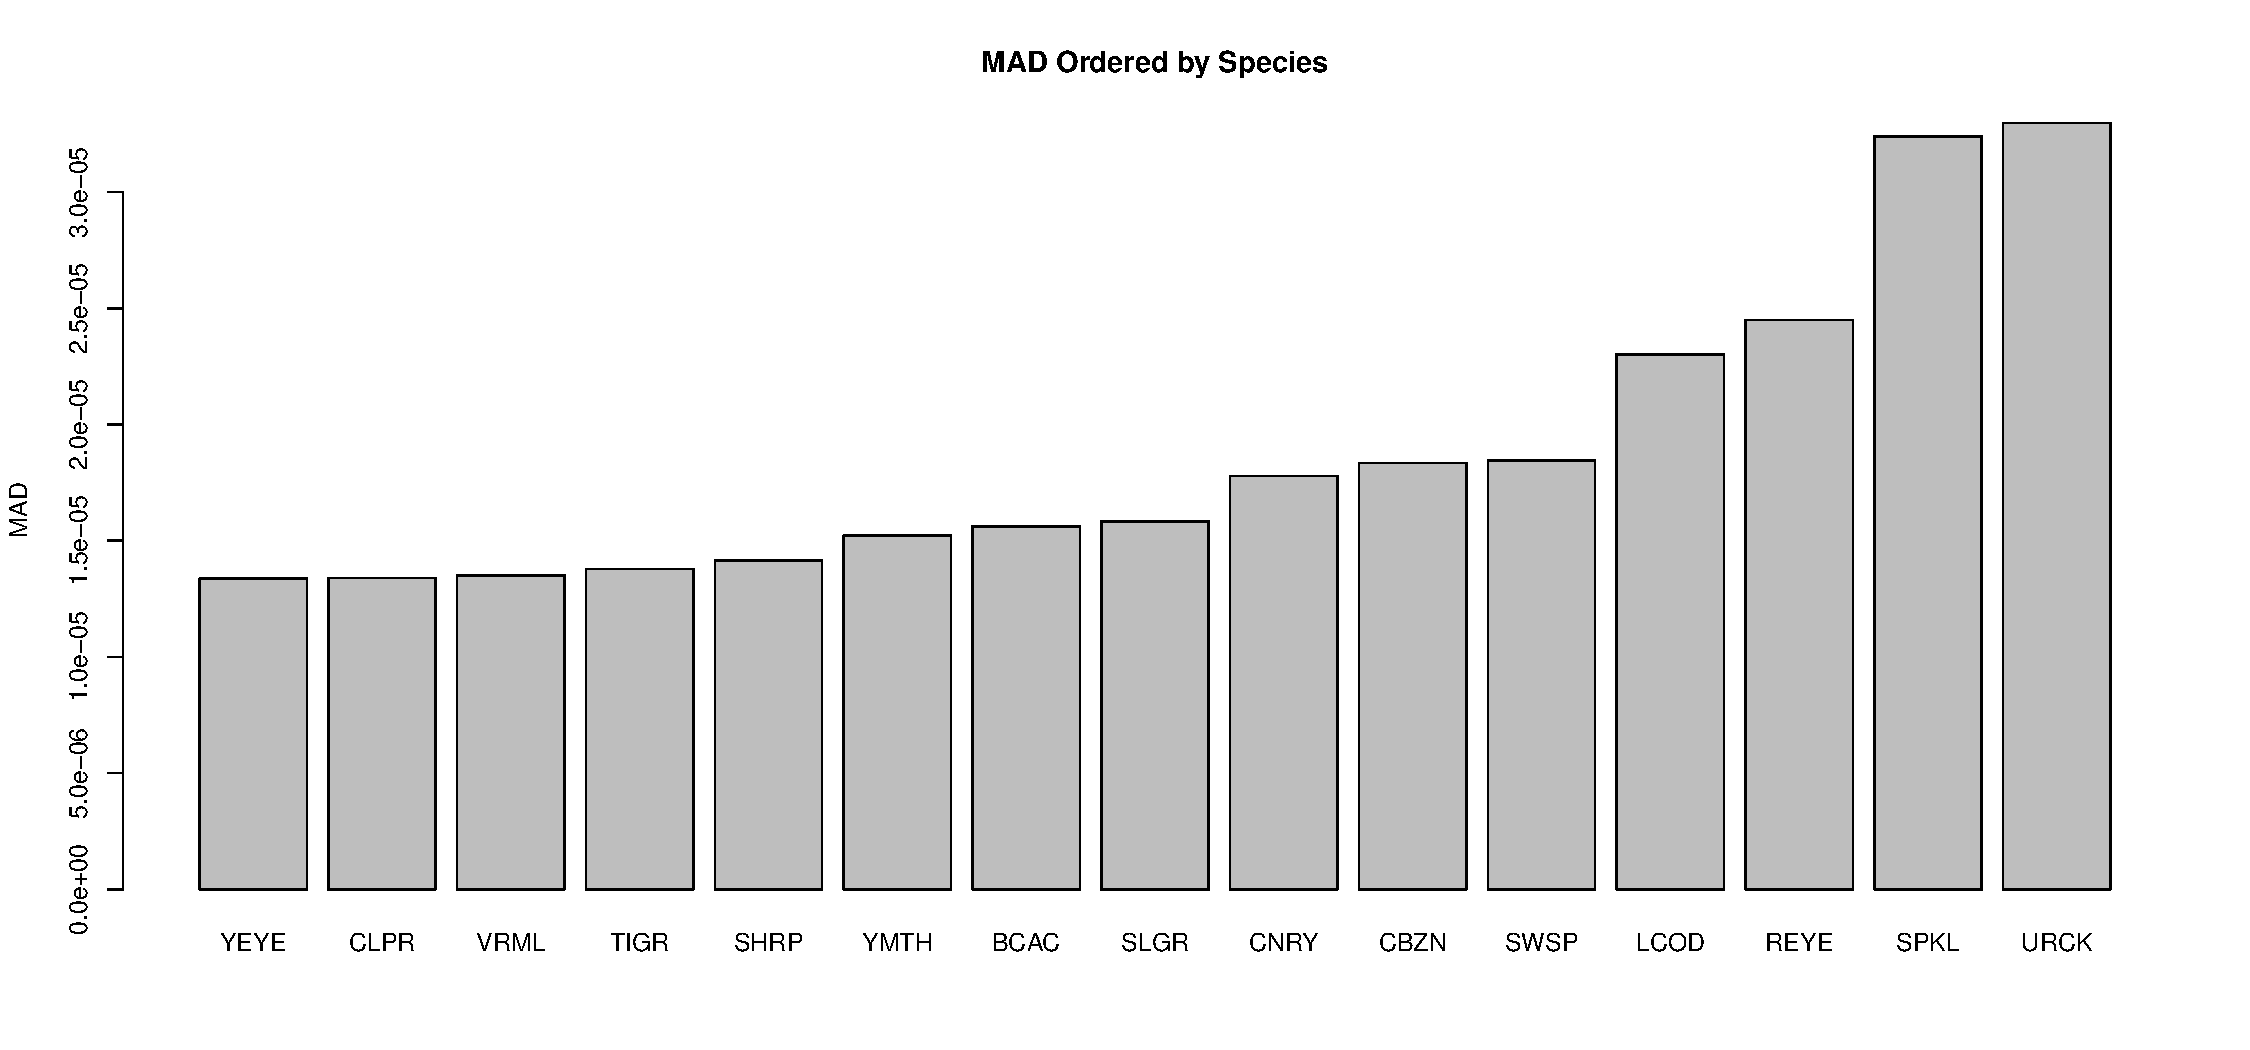
\includegraphics[width=1\textwidth]{../sscRuns/25019781982M3/sppMad95.pdf}
%	%\end{figure}
%%	
%%	\begin{itemize}
%%	\item metrics
%%	\item focus on a couple model to compare ()
%%	\item look at sppMad68
%%	\item consider a couple of the best and worst marginals
%%	\end{itemize}
%
%\clearpage
%\subsubsection{M4}
%	\begin{figure}[ht!]
%	\centering
%	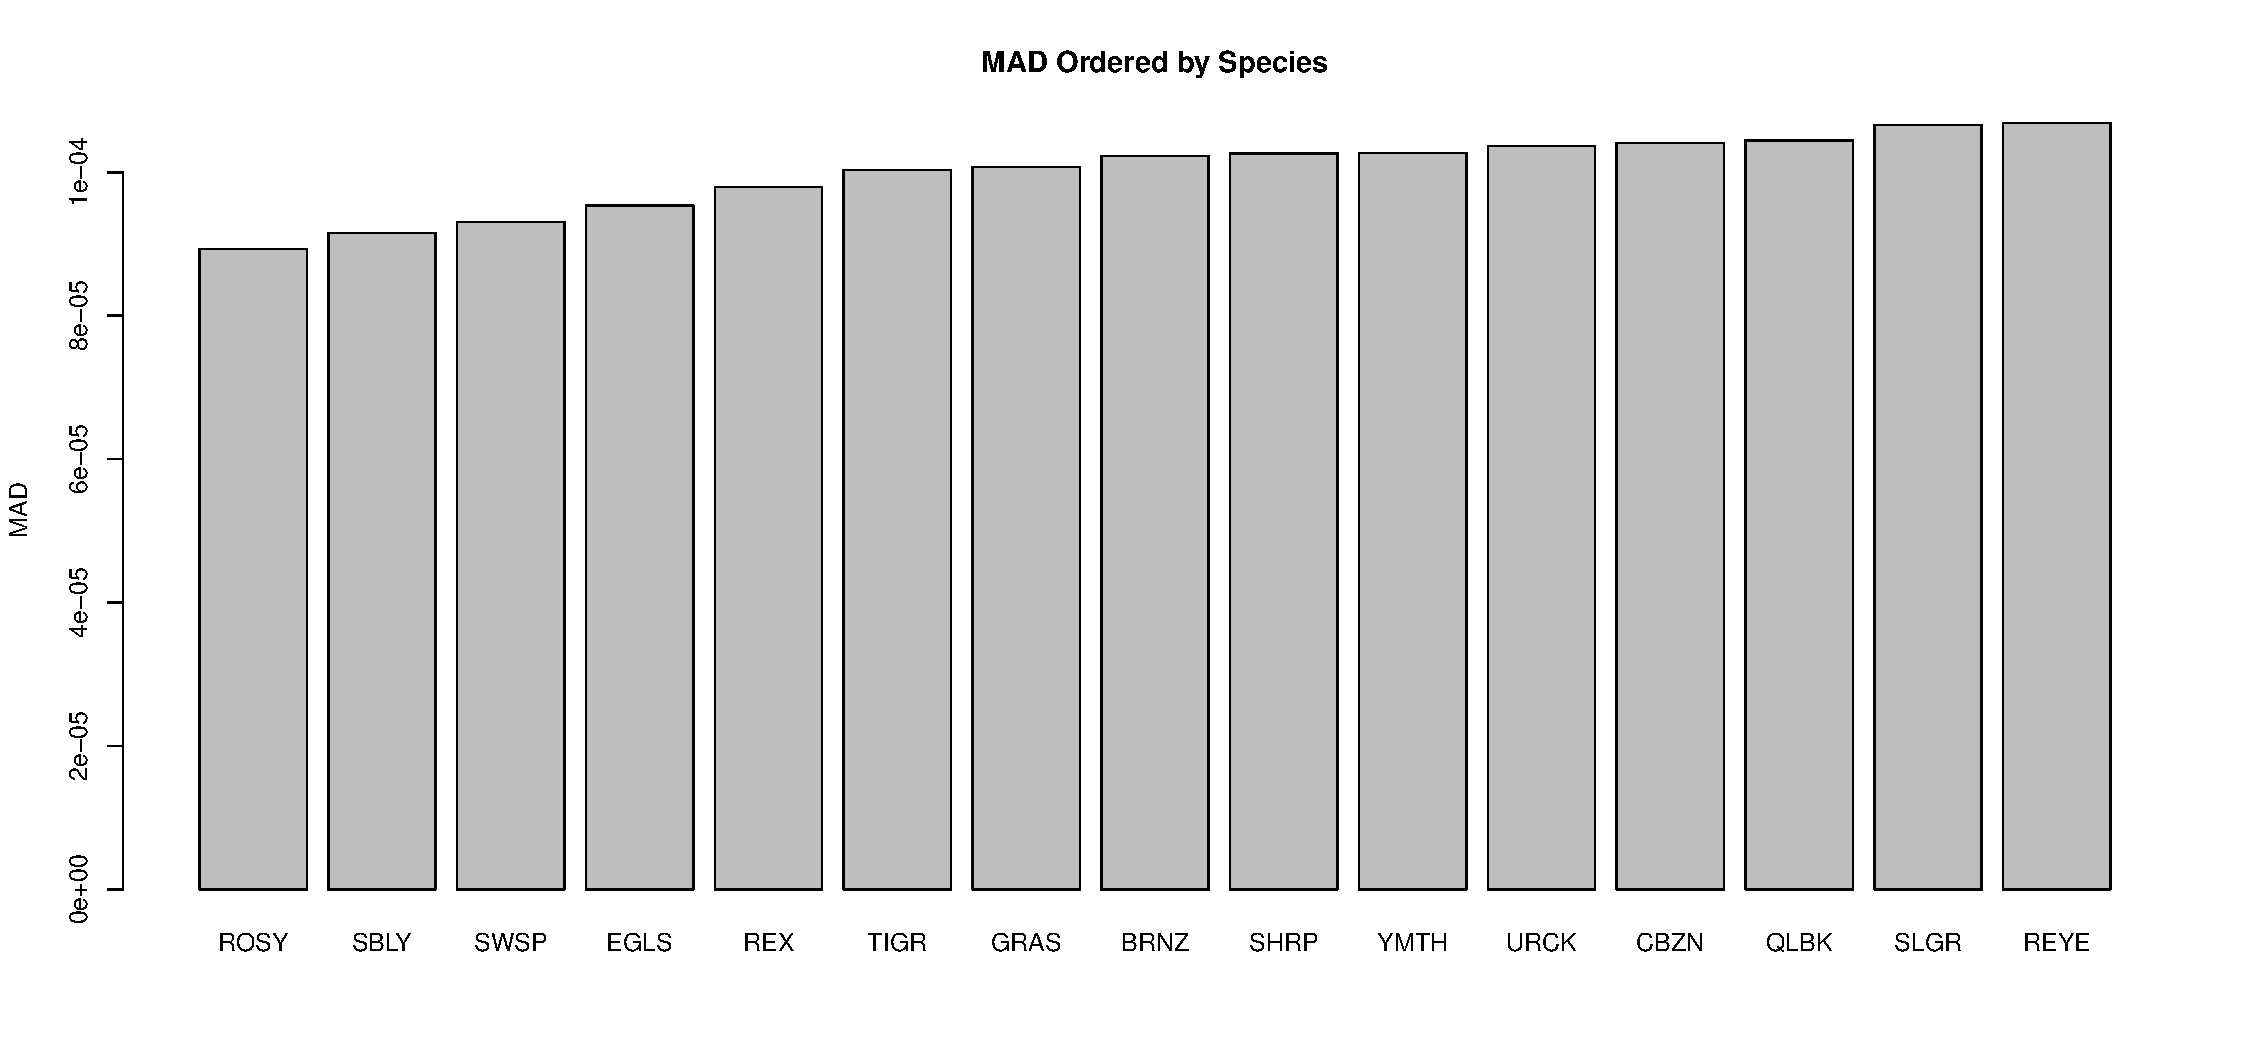
\includegraphics[width=1\textwidth]{../sscRuns/25019781982M4/sppMad68.pdf}
%	\end{figure}
%
%	\begin{figure}[ht!]
%	\centering
%	\includegraphics[width=1.1\textwidth]{{../sscRuns/25019781982M4/marginalRDBD/marginalRDBD-0.68-Diagnostic}.pdf}
%	\end{figure}
%
%	\begin{figure}[ht!]
%	\centering
%	\includegraphics[width=1.1\textwidth]{{../sscRuns/25019781982M4/marginalWDOW/marginalWDOW-0.68-Diagnostic}.pdf}
%	\end{figure}
%	
%	\begin{figure}[ht!]
%	\centering
%	\includegraphics[width=1.1\textwidth]{{../sscRuns/25019781982M4/marginalROSY/marginalROSY-0.68-Diagnostic}.pdf}
%	\end{figure}
%
%	\begin{figure}[ht!]
%	\centering
%	\includegraphics[width=1.1\textwidth]{{../sscRuns/25019781982M4/marginalREYE/marginalREYE-0.68-Diagnostic}.pdf}
%	\end{figure}	
%
%\clearpage
%\subsubsection{M6}
%	\begin{figure}[ht!]
%	\centering
%	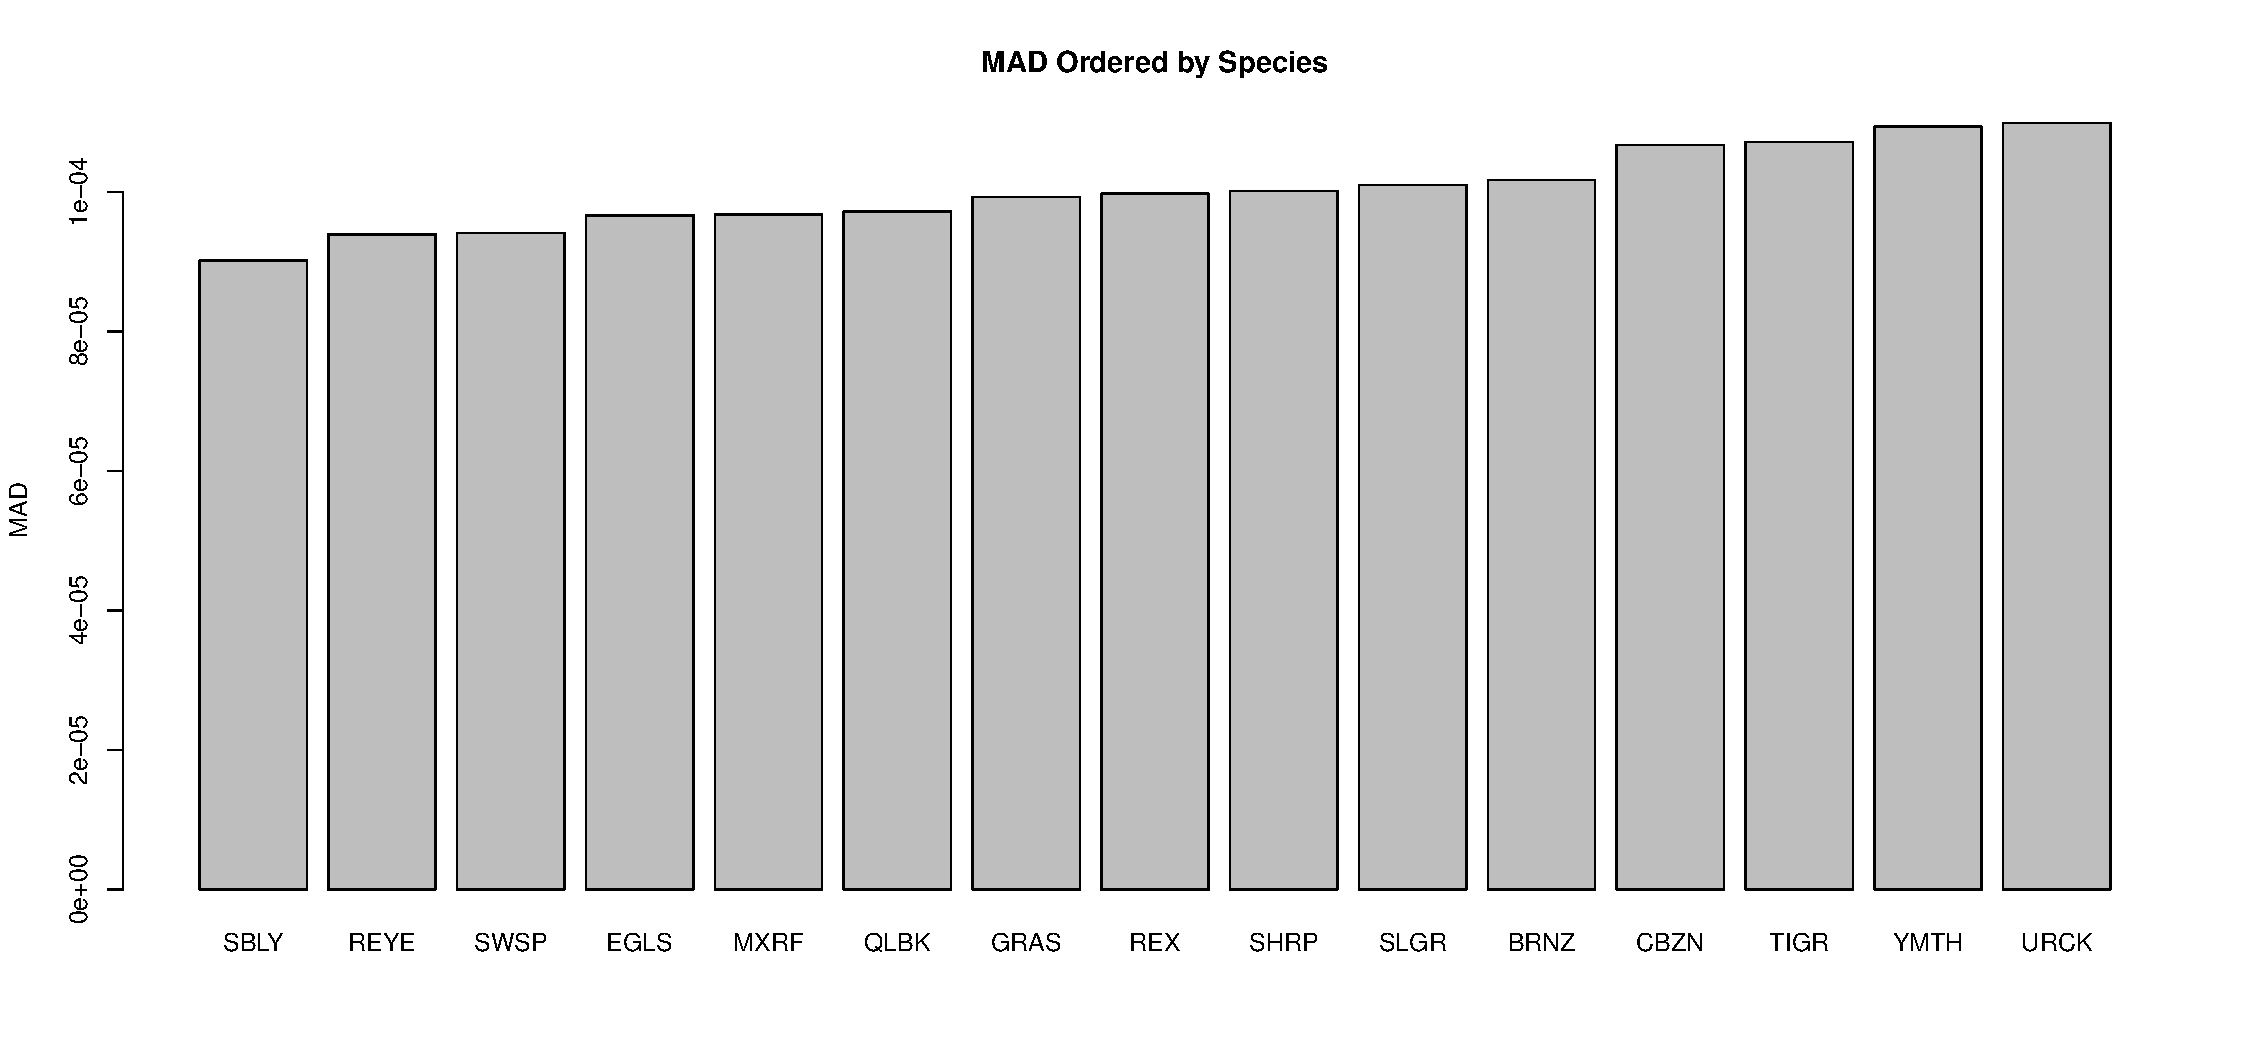
\includegraphics[width=1\textwidth]{../sscRuns/25019781982M6/sppMad68.pdf}
%	\end{figure}
%
%	\begin{figure}[ht!]
%	\centering
%	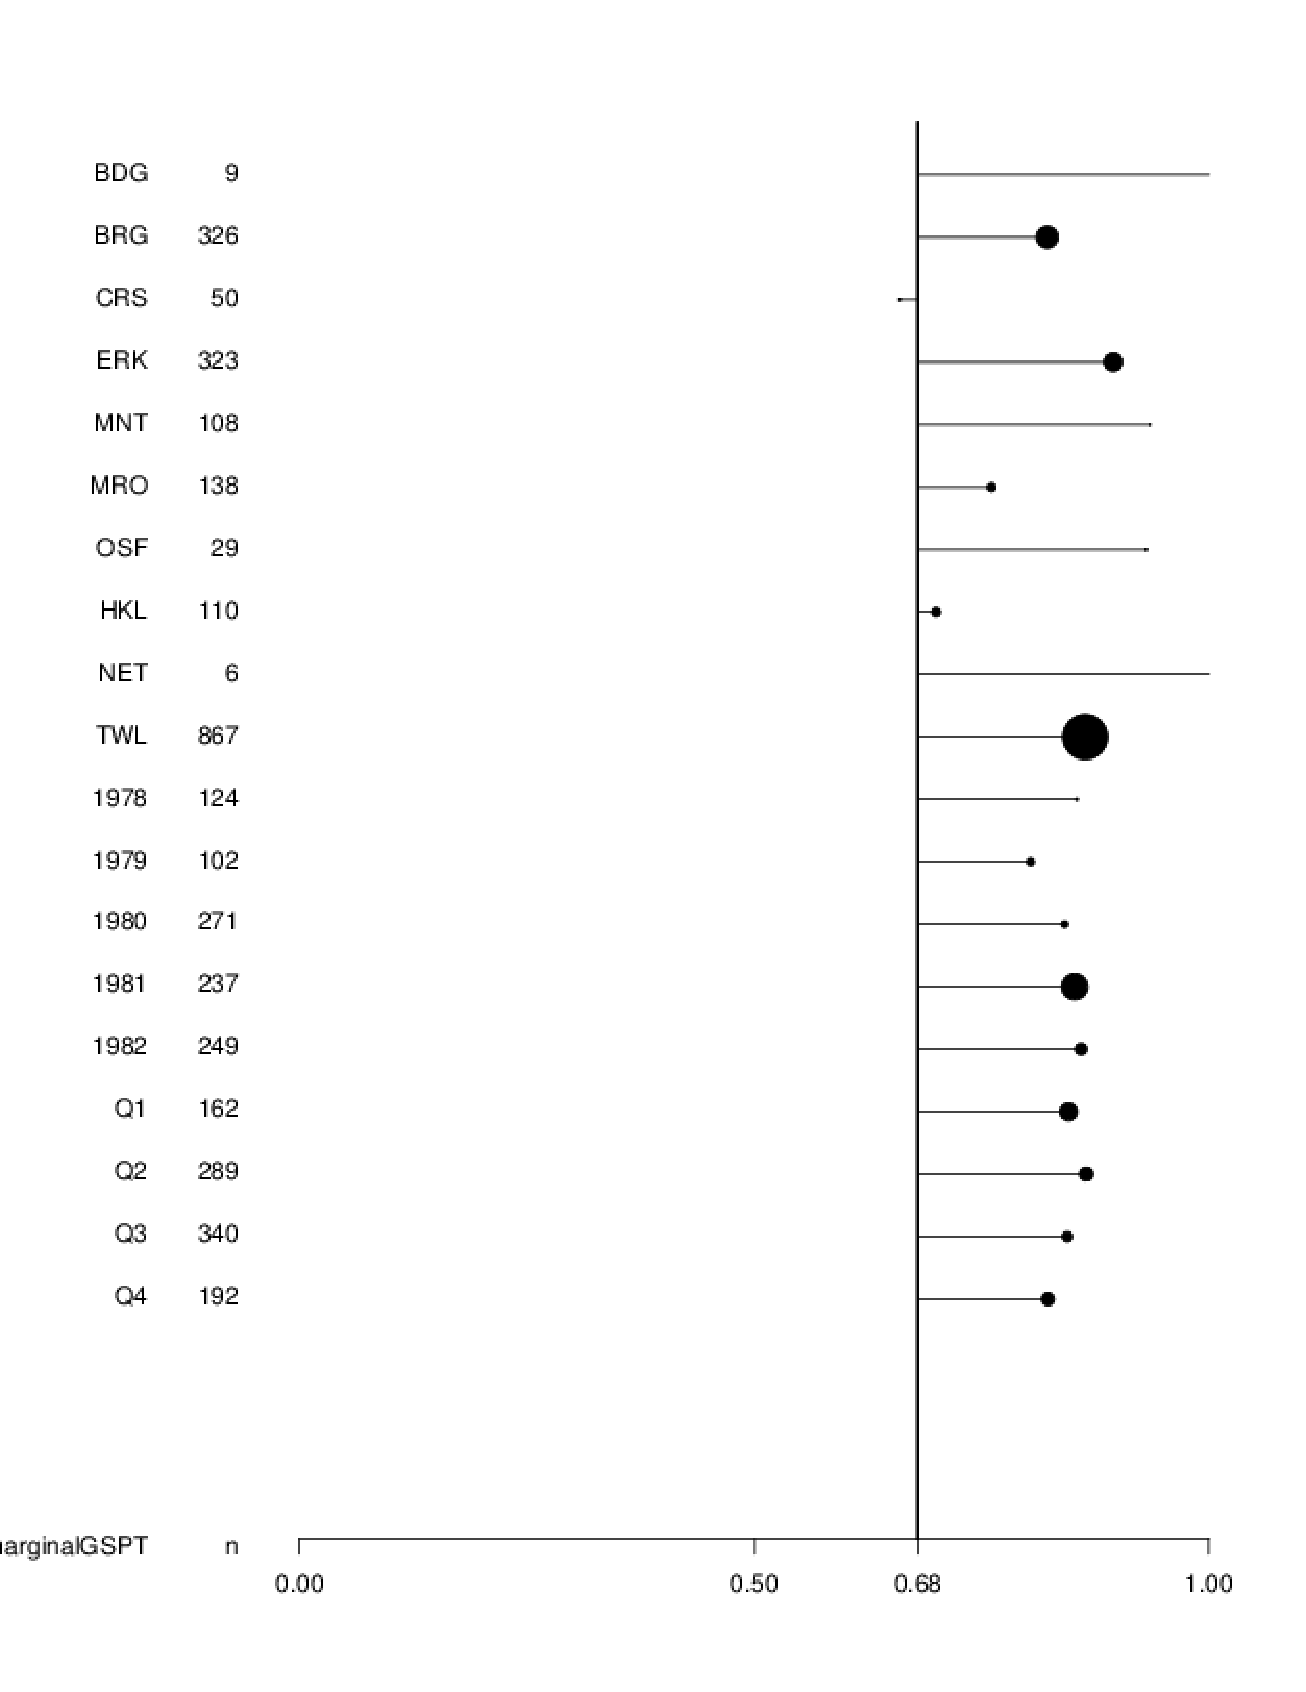
\includegraphics[width=1.1\textwidth]{{../sscRuns/25019781982M6/marginalGSPT/marginalGSPT-0.68-Diagnostic}.pdf}
%	\end{figure}
%
%	\begin{figure}[ht!]
%	\centering
%	\includegraphics[width=1.1\textwidth]{{../sscRuns/25019781982M6/marginalWDOW/marginalWDOW-0.68-Diagnostic}.pdf}
%	\end{figure}
%	
%	\begin{figure}[ht!]
%	\centering
%	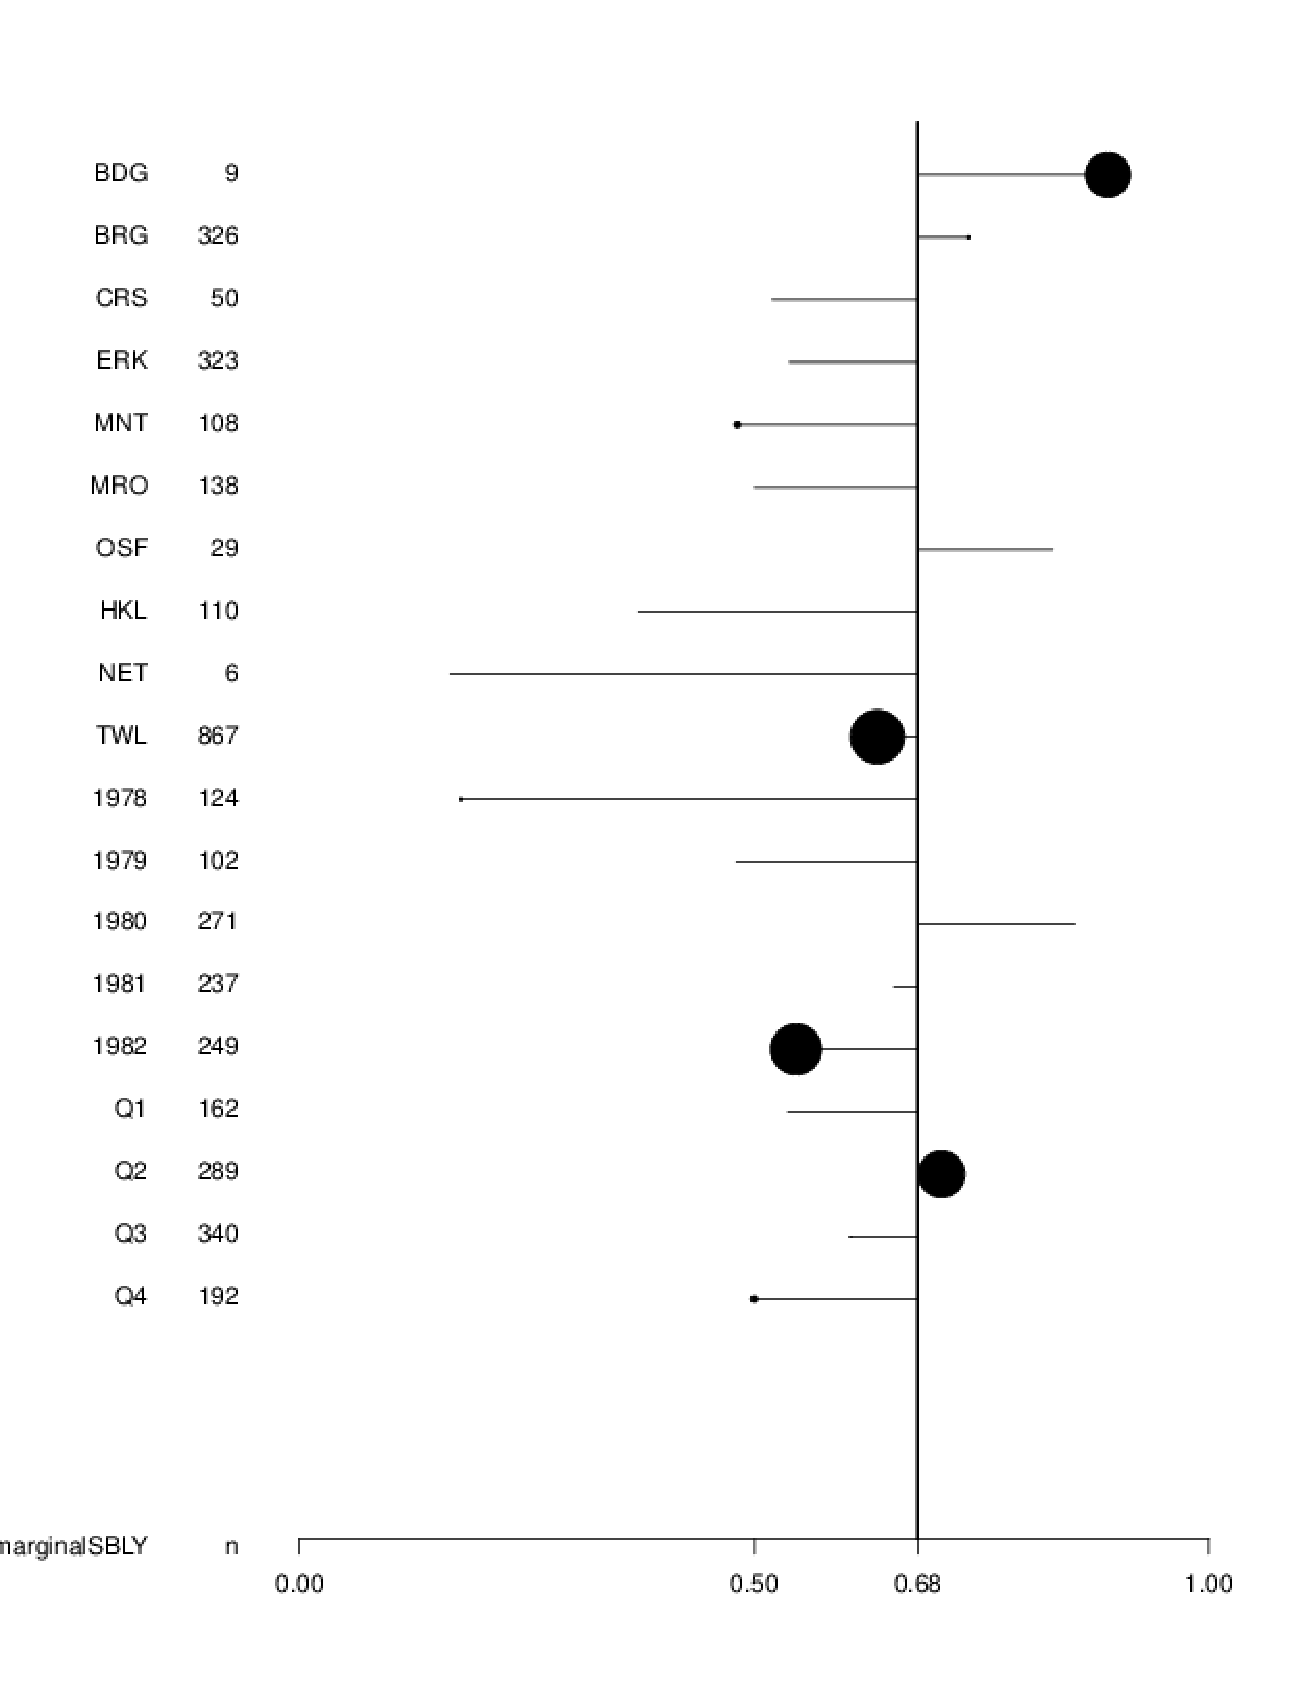
\includegraphics[width=1.1\textwidth]{{../sscRuns/25019781982M6/marginalSBLY/marginalSBLY-0.68-Diagnostic}.pdf}
%	\end{figure}
%
%	\begin{figure}[ht!]
%	\centering
%	\includegraphics[width=1.1\textwidth]{{../sscRuns/25019781982M6/marginalURCK/marginalURCK-0.68-Diagnostic}.pdf}
%	\end{figure}

\clearpage
\subsection{MCAT 250 Priors}
	\begin{table}[ht!]
        \centering
        \begin{tabular}[c]{@{}lcccccc@{}}
        %\toprule
        \hline
        & M4HC1 & M4HC3 & M4U4 \\ \hline
        \(\Delta\) DIC & 0.02 & 0.1 & 0 \\                                                
	\(\Delta\) WAIC & 0.03 & 0.11 & 0 \\                                              
	\(pr(M|y)\) & 0.21 & 0.37 & 0.42
        \end{tabular}
        \end{table}

\subsubsection{\href{https://github.com/gasduster99/sppComp/tree/master/sscRuns/25019781982M4HC1}{M4HC1}, \href{https://github.com/gasduster99/sppComp/tree/master/sscRuns/25019781982M4HC3}{M4HC3}, \href{https://github.com/gasduster99/sppComp/tree/master/sscRuns/25019781982M4U4}{M4U4} \href{https://github.com/gasduster99/sppComp/tree/master/try1/postSSC/25019781982M4HC1HC3U4}{Comparision}}
	\begin{figure}[ht!]
	\centering
	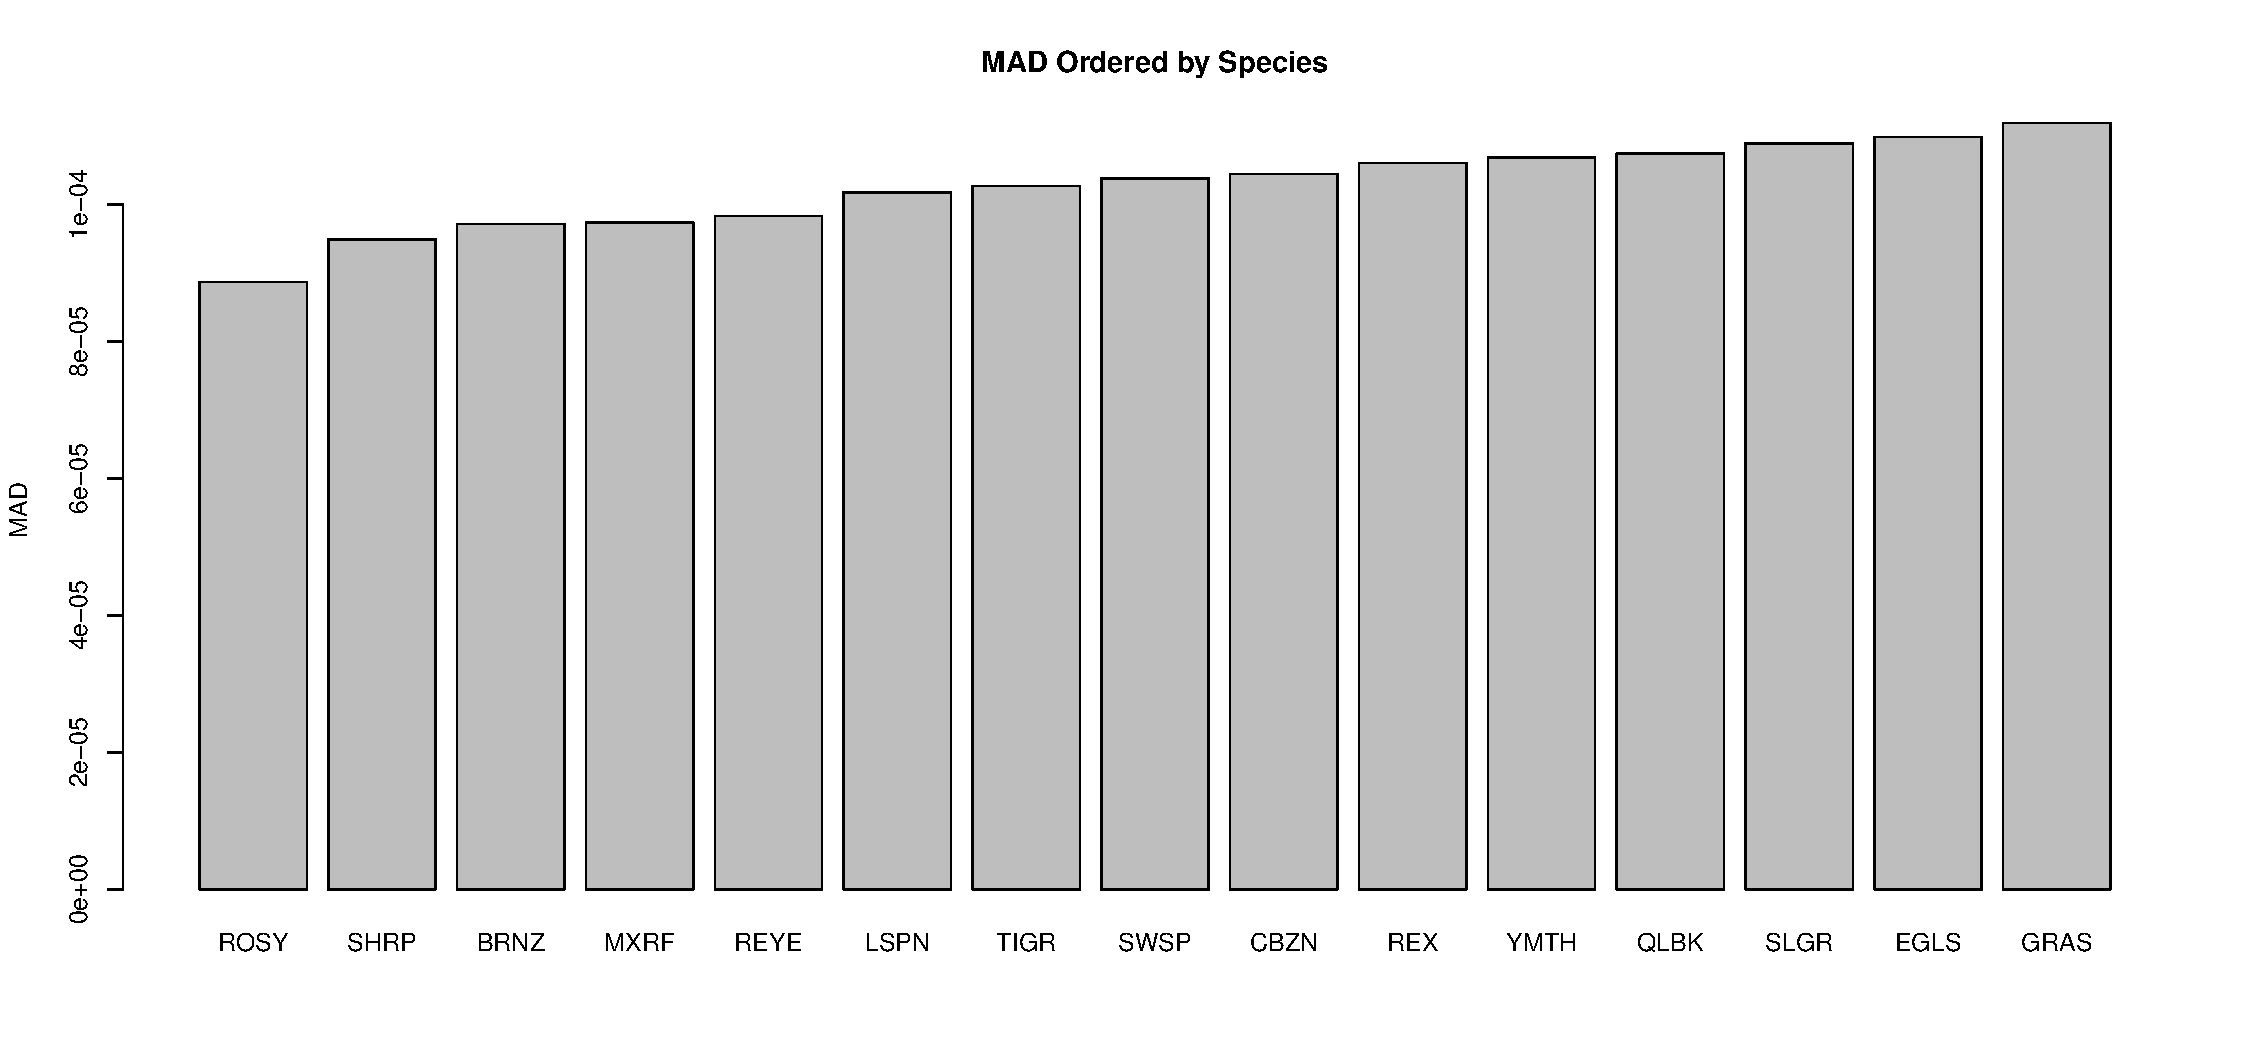
\includegraphics[width=0.6\textwidth]{../sscRuns/25019781982M4HC1/sppMad68.pdf}
	\end{figure}

	\begin{figure}[ht!]
	\centering
	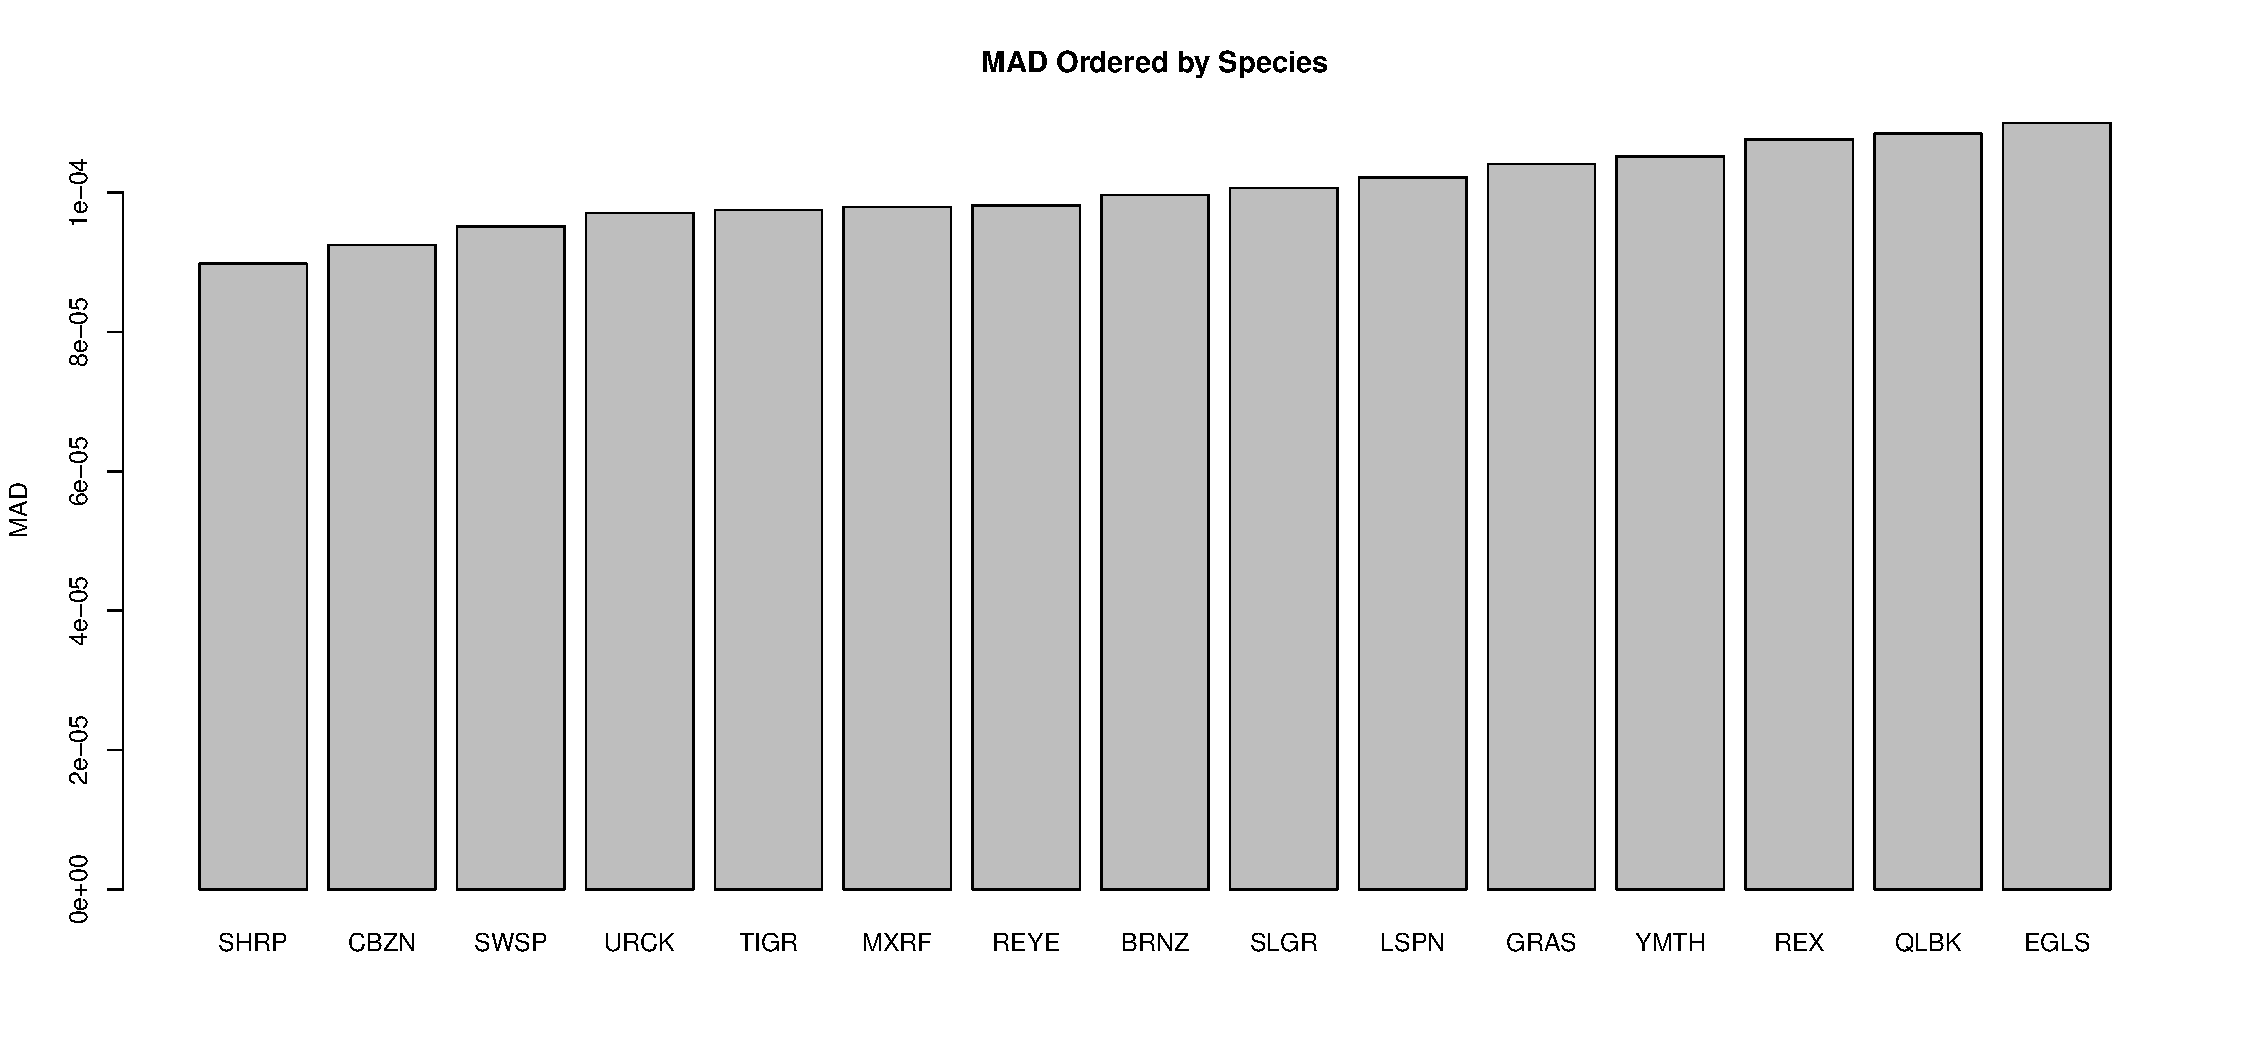
\includegraphics[width=0.6\textwidth]{../sscRuns/25019781982M4HC3/sppMad68.pdf}
	\end{figure}
	
	\begin{figure}[ht!]
	\centering
	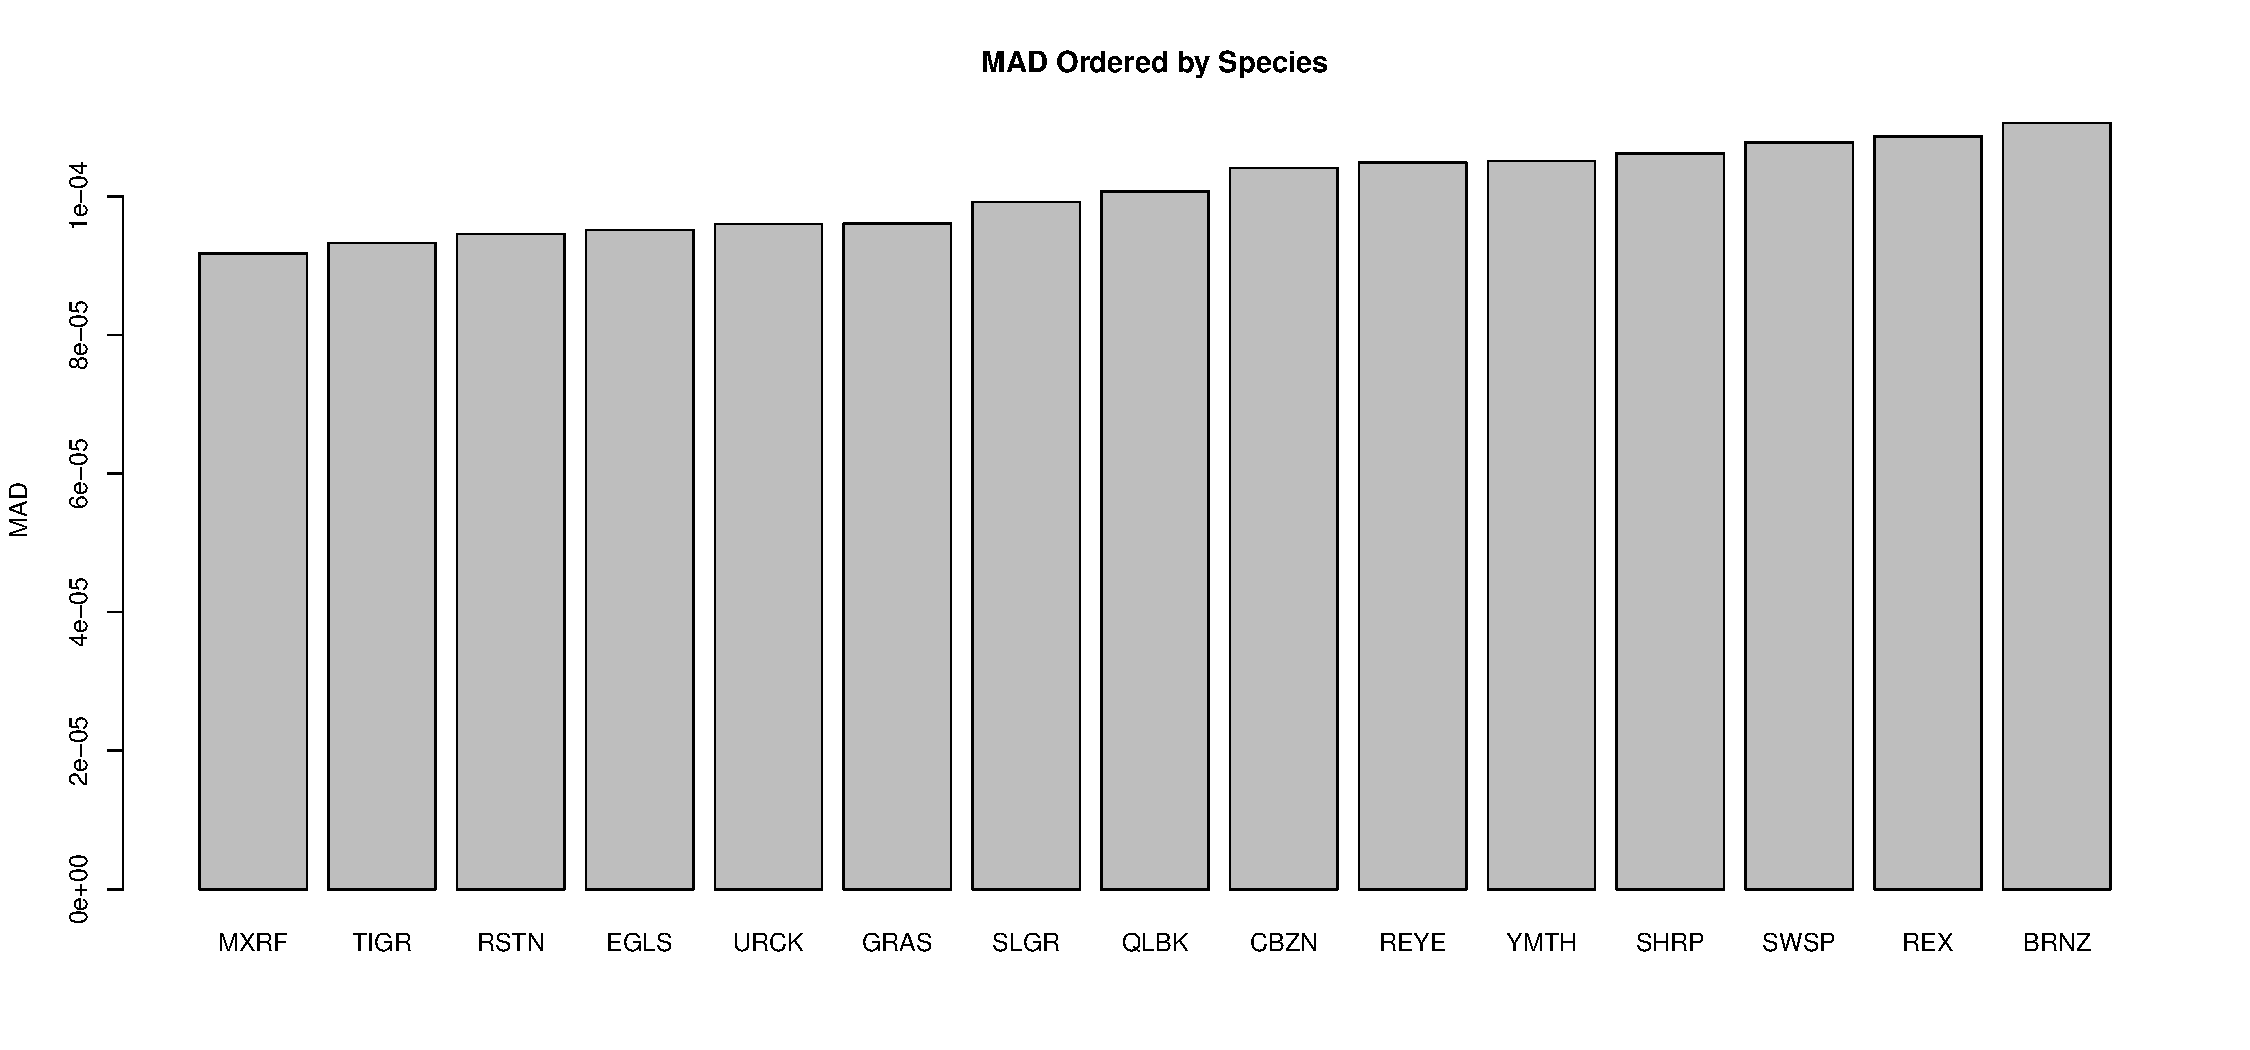
\includegraphics[width=0.6\textwidth]{../sscRuns/25019781982M4U4/sppMad68.pdf}
	\end{figure}

	\clearpage
        \begin{figure}[ht!]
        \centering
        \includegraphics[width=1.1\textwidth]{{./postSSC/25019781982M4HC1HC3U4/marginalBCAC/marginalBCAC-0.68-Diagnostic}.pdf}
        \end{figure}

	\clearpage
        \begin{figure}[ht!]
        \centering
        \includegraphics[width=1.1\textwidth]{{./postSSC/25019781982M4HC1HC3U4/marginalWDOW/marginalWDOW-0.68-Diagnostic}.pdf}
        \end{figure}

	\clearpage
        \begin{figure}[ht!]
        \centering
        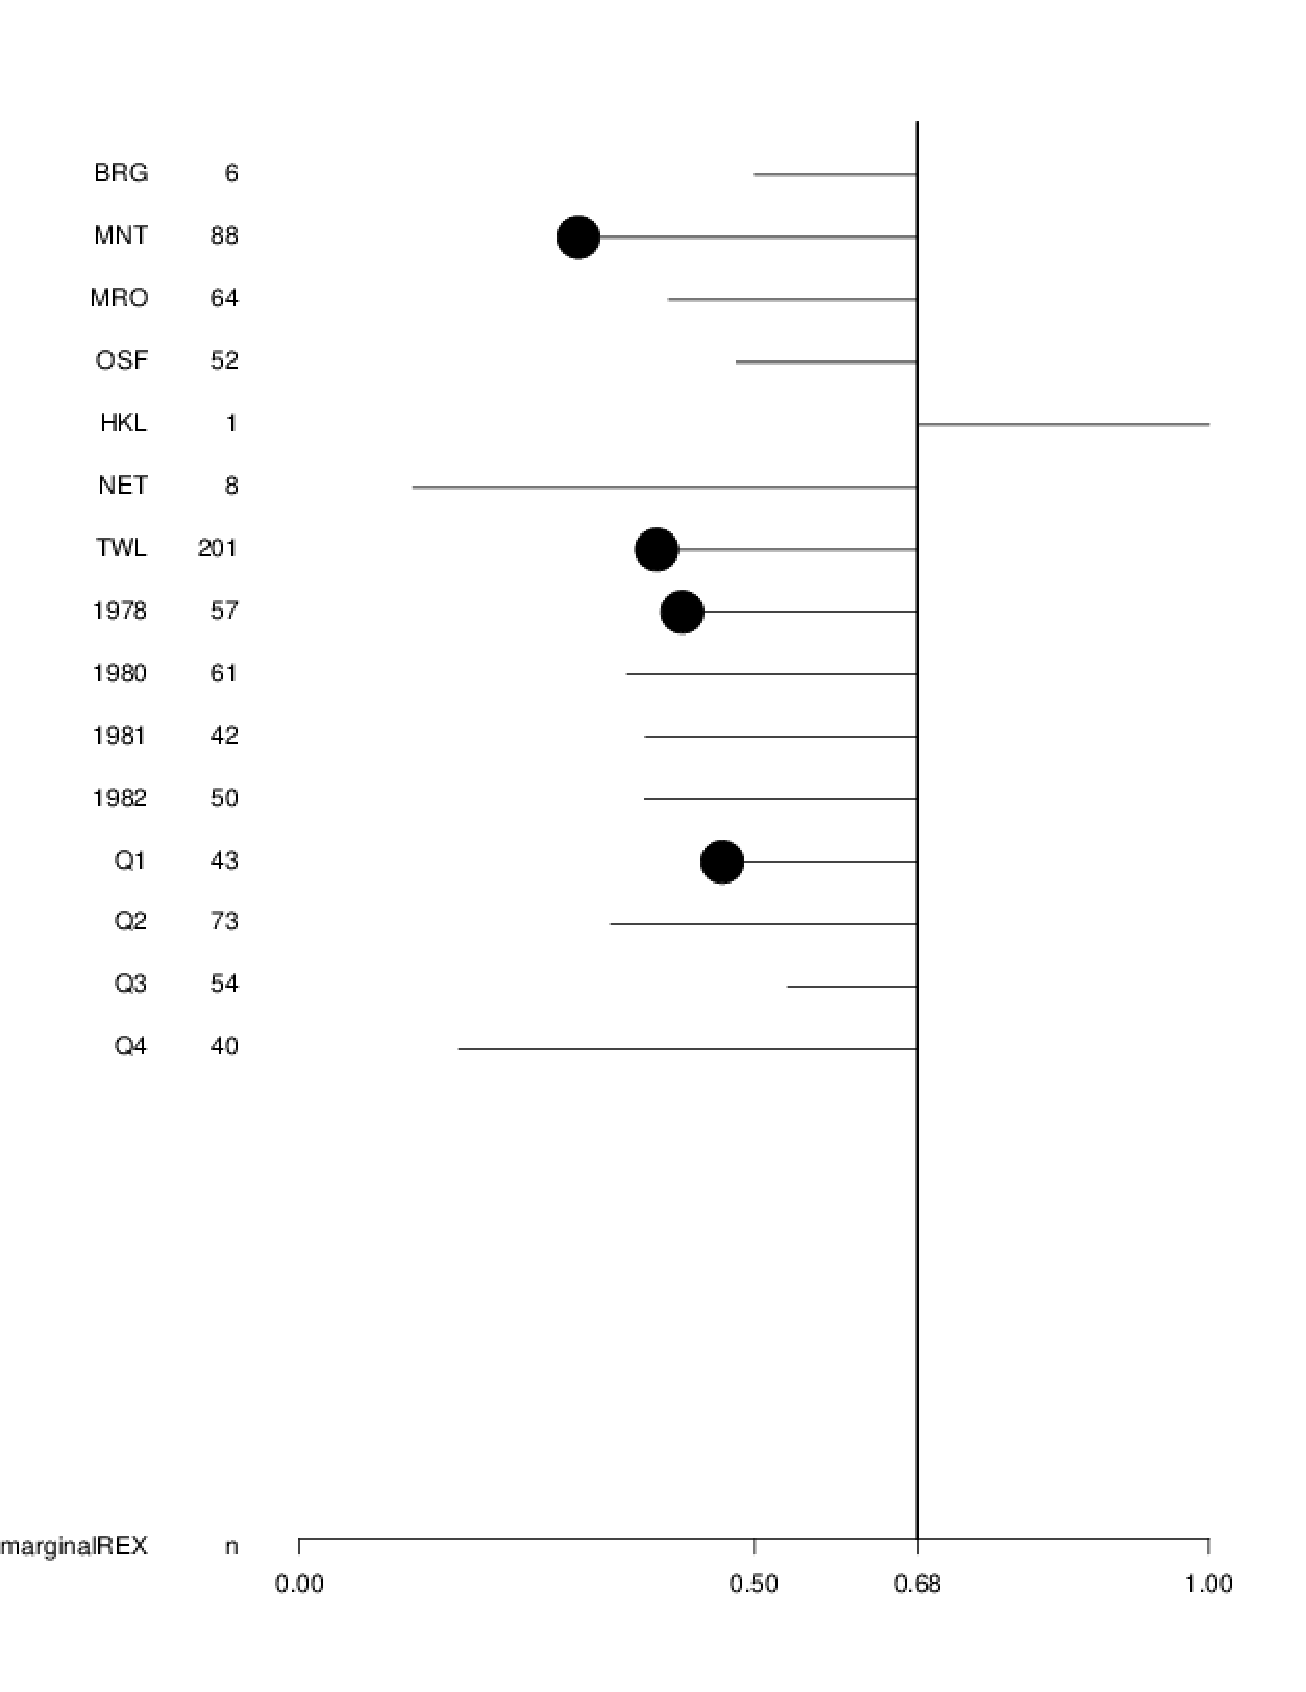
\includegraphics[width=1.1\textwidth]{{./postSSC/25019781982M4HC1HC3U4/marginalREX/marginalREX-0.68-Diagnostic}.pdf}
        \end{figure}

	\clearpage
        \begin{figure}[ht!]
        \centering
        \includegraphics[width=1.1\textwidth]{{./postSSC/25019781982M4HC1HC3U4/marginalBRNZ/marginalBRNZ-0.68-Diagnostic}.pdf}
        \end{figure}


%	\begin{figure}[ht!]
%	\centering
%	\includegraphics[width=0.8\textwidth]{{../sscRuns/25019781982M4HC1/marginalRDBD/marginalRDBD-0.68-Diagnostic}.pdf}
%	\end{figure}
%
%	\begin{figure}[ht!]
%	\centering
%	\includegraphics[width=1.1\textwidth]{{../sscRuns/25019781982M4HC1/marginalWDOW/marginalWDOW-0.68-Diagnostic}.pdf}
%	\end{figure}
%	
%	\begin{figure}[ht!]
%	\centering
%	\includegraphics[width=1.1\textwidth]{{../sscRuns/25019781982M4HC1/marginalROSY/marginalROSY-0.68-Diagnostic}.pdf}
%	\end{figure}
%
%	\begin{figure}[ht!]
%	\centering
%	\includegraphics[width=1.1\textwidth]{{../sscRuns/25019781982M4HC1/marginalREYE/marginalREYE-0.68-Diagnostic}.pdf}
%	\end{figure}
%
%\clearpage
%\subsubsection{M4HC3}
%	%\begin{figure}[ht!]
%	%\centering
%	%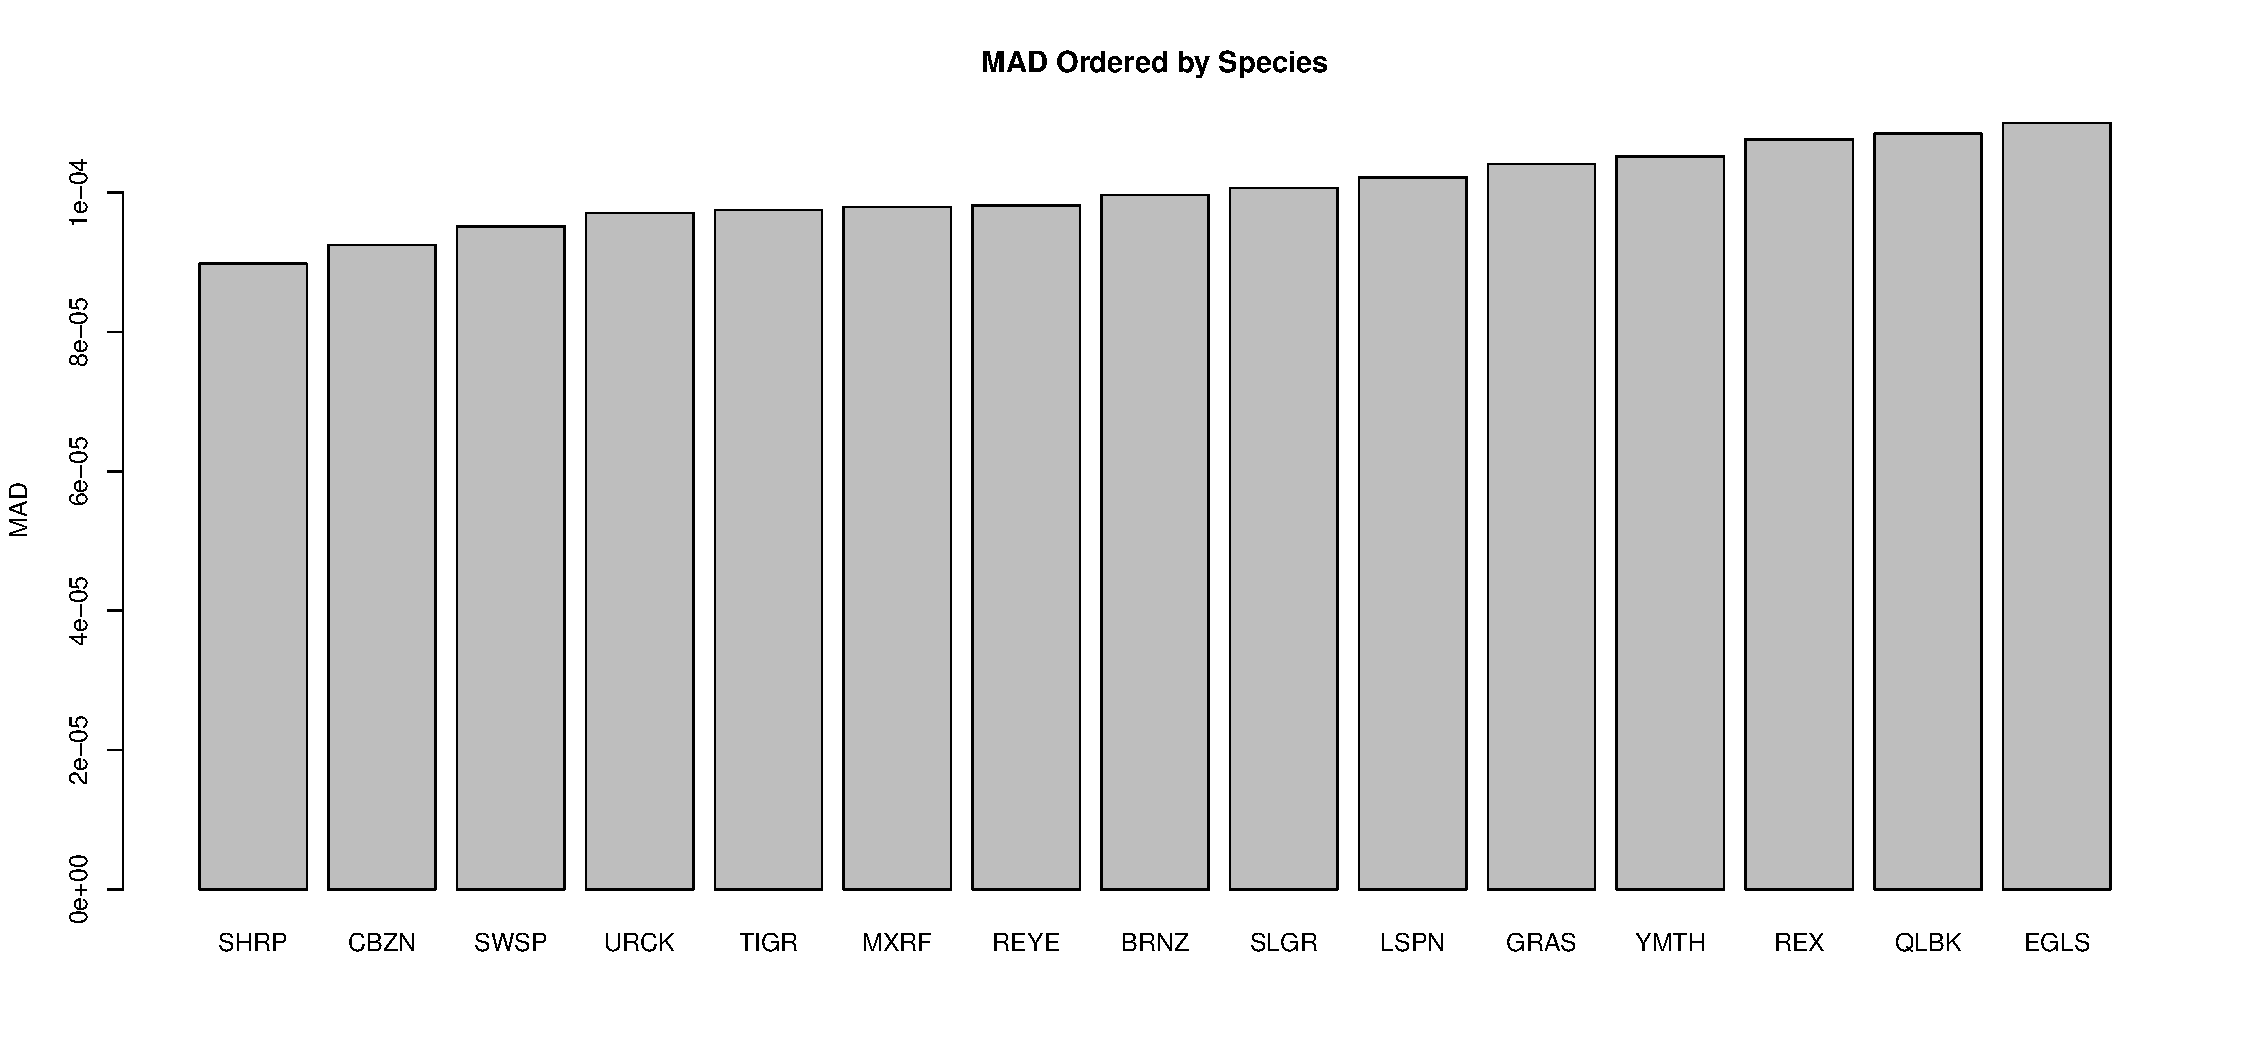
\includegraphics[width=1\textwidth]{../sscRuns/25019781982M4HC3/sppMad68.pdf}
%	%\end{figure}
%
%	\begin{figure}[ht!]
%	\centering
%	\includegraphics[width=0.9\textwidth]{{../sscRuns/25019781982M4HC3/marginalRDBD/marginalRDBD-0.68-Diagnostic}.pdf}
%	\end{figure}
%
%	\begin{figure}[ht!]
%	\centering
%	\includegraphics[width=1.1\textwidth]{{../sscRuns/25019781982M4HC3/marginalWDOW/marginalWDOW-0.68-Diagnostic}.pdf}
%	\end{figure}
%	
%	\begin{figure}[ht!]
%	\centering
%	\includegraphics[width=1.1\textwidth]{{../sscRuns/25019781982M4HC3/marginalROSY/marginalROSY-0.68-Diagnostic}.pdf}
%	\end{figure}
%
%	\begin{figure}[ht!]
%	\centering
%	\includegraphics[width=1.1\textwidth]{{../sscRuns/25019781982M4HC3/marginalREYE/marginalREYE-0.68-Diagnostic}.pdf}
%	\end{figure}
%
%\clearpage
%\subsubsection{M4U4}
%	%\begin{figure}[ht!]
%	%\centering
%	%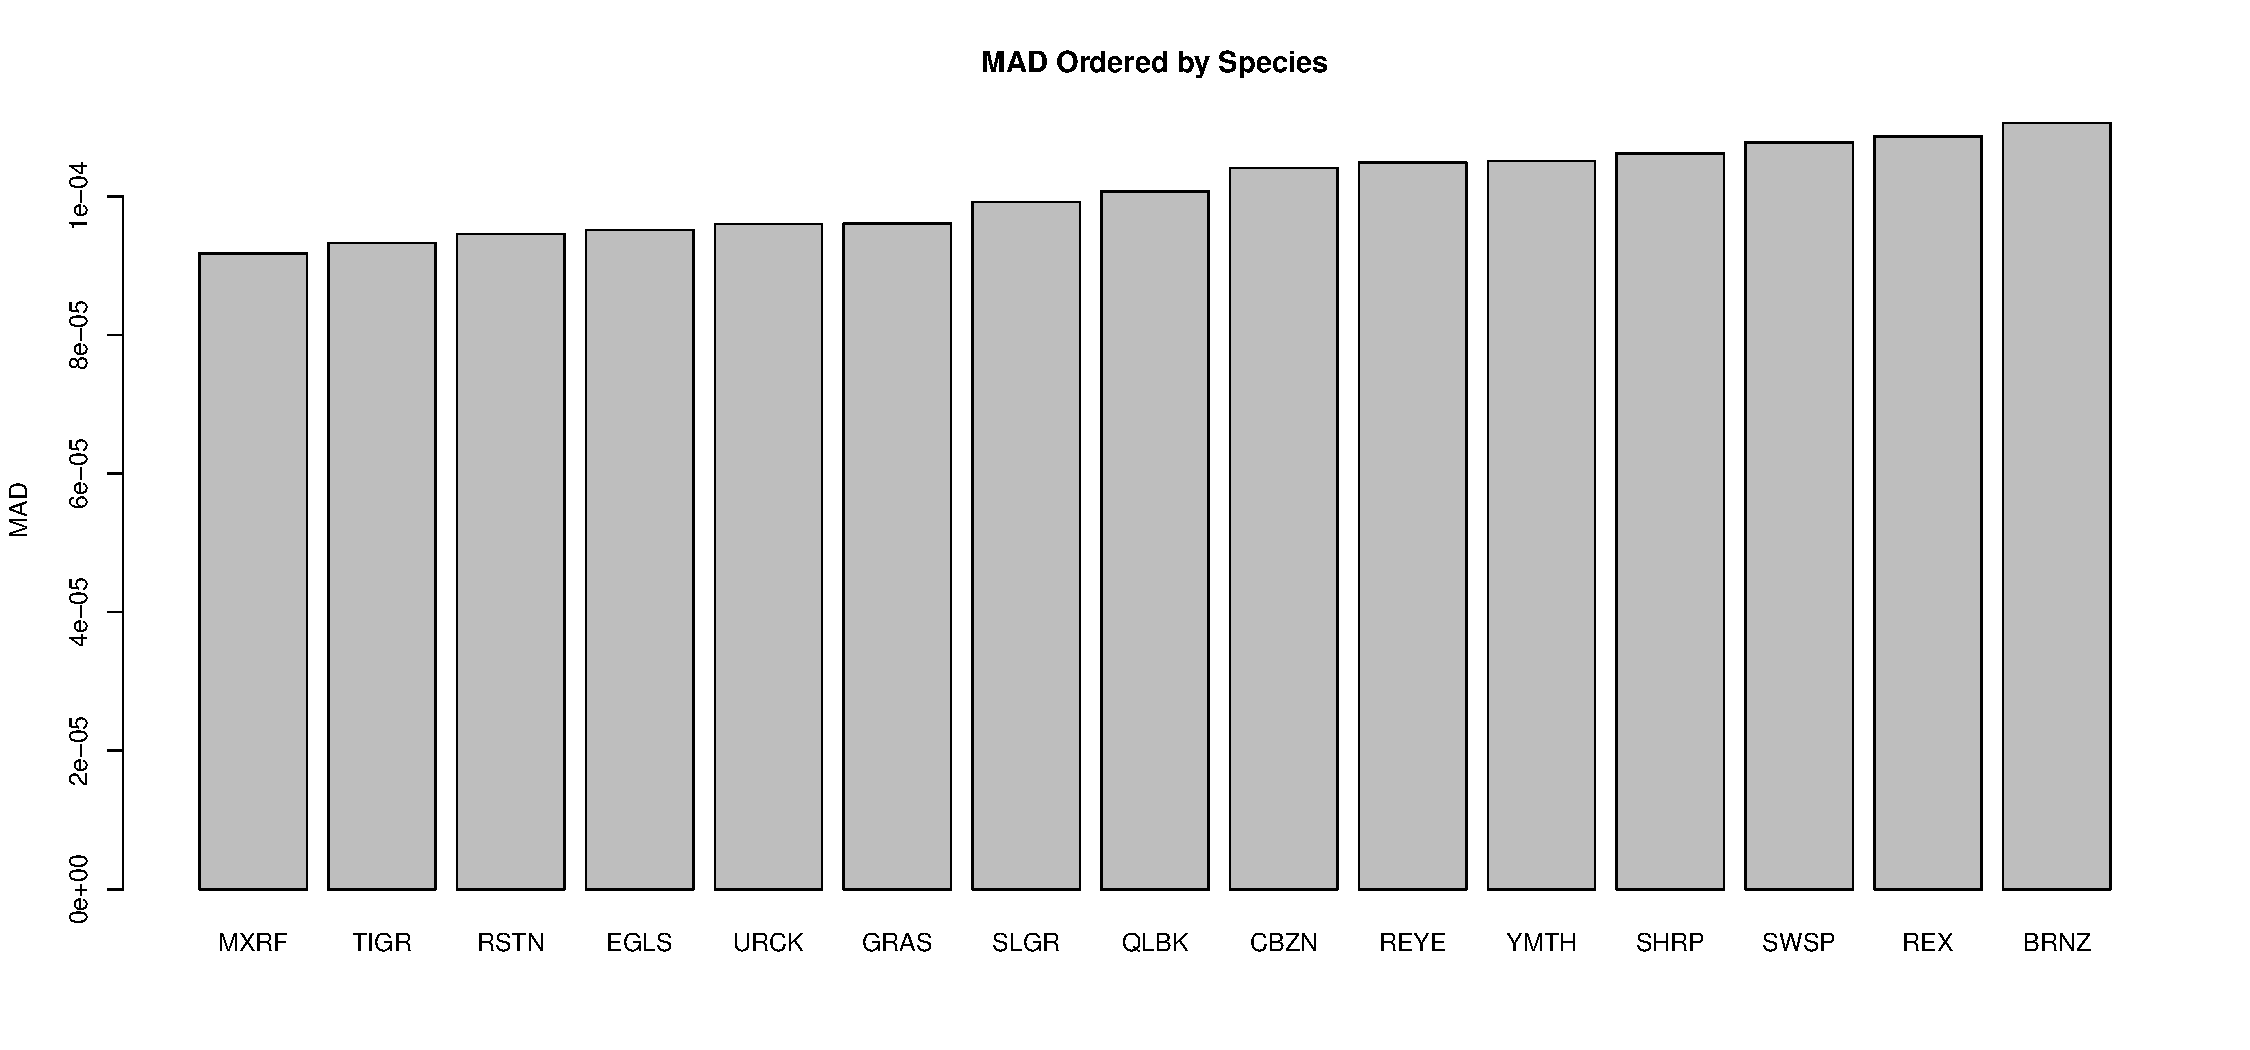
\includegraphics[width=1\textwidth]{../sscRuns/25019781982M4U4/sppMad68.pdf}
%	%\end{figure}
%
%	\begin{figure}[ht!]
%	\centering
%	\includegraphics[width=0.9\textwidth]{{../sscRuns/25019781982M4U4/marginalRDBD/marginalRDBD-0.68-Diagnostic}.pdf}
%	\end{figure}
%
%	\begin{figure}[ht!]
%	\centering
%	\includegraphics[width=1.1\textwidth]{{../sscRuns/25019781982M4U4/marginalWDOW/marginalWDOW-0.68-Diagnostic}.pdf}
%	\end{figure}
%	
%	\begin{figure}[ht!]
%	\centering
%	\includegraphics[width=1.1\textwidth]{{../sscRuns/25019781982M4U4/marginalROSY/marginalROSY-0.68-Diagnostic}.pdf}
%	\end{figure}
%
%	\begin{figure}[ht!]
%	\centering
%	\includegraphics[width=1.1\textwidth]{{../sscRuns/25019781982M4U4/marginalREYE/marginalREYE-0.68-Diagnostic}.pdf}
%	\end{figure}
	
\clearpage
\subsection{MCAT 253 Time Models}
	\begin{table}[h!]
	\centering
	\begin{tabular}[c]{@{}lcccccc@{}}
	%\toprule
	\hline
	& M1 & M2 & M3 & M4 & M5 & M6 \\ \hline
	\(\Delta\) DIC & 1409.81 & 0.09 & 0.1 & 0.07 & 0.05 & 0 \\
	\(\Delta\) WAIC & 1391.66 & 0.16 & 0.18 & 0 & 0.13 & 0.08 \\
	\(pr(M|y)\) & 0 & 0 & 0 & 1 & 0 & 0	
	\end{tabular}
	\end{table}

\subsection{\href{https://github.com/gasduster99/sppComp/tree/master/sscRuns/25319781982M4}{M4}, \href{https://github.com/gasduster99/sppComp/tree/master/sscRuns/25319781982M5}{M5}, \href{https://github.com/gasduster99/sppComp/tree/master/sscRuns/25319781982M6}{M6} \href{https://github.com/gasduster99/sppComp/tree/master/try1/postSSC/25319781982M4M5M6}{Comparision}}
	\begin{figure}[ht!]
        \centering
        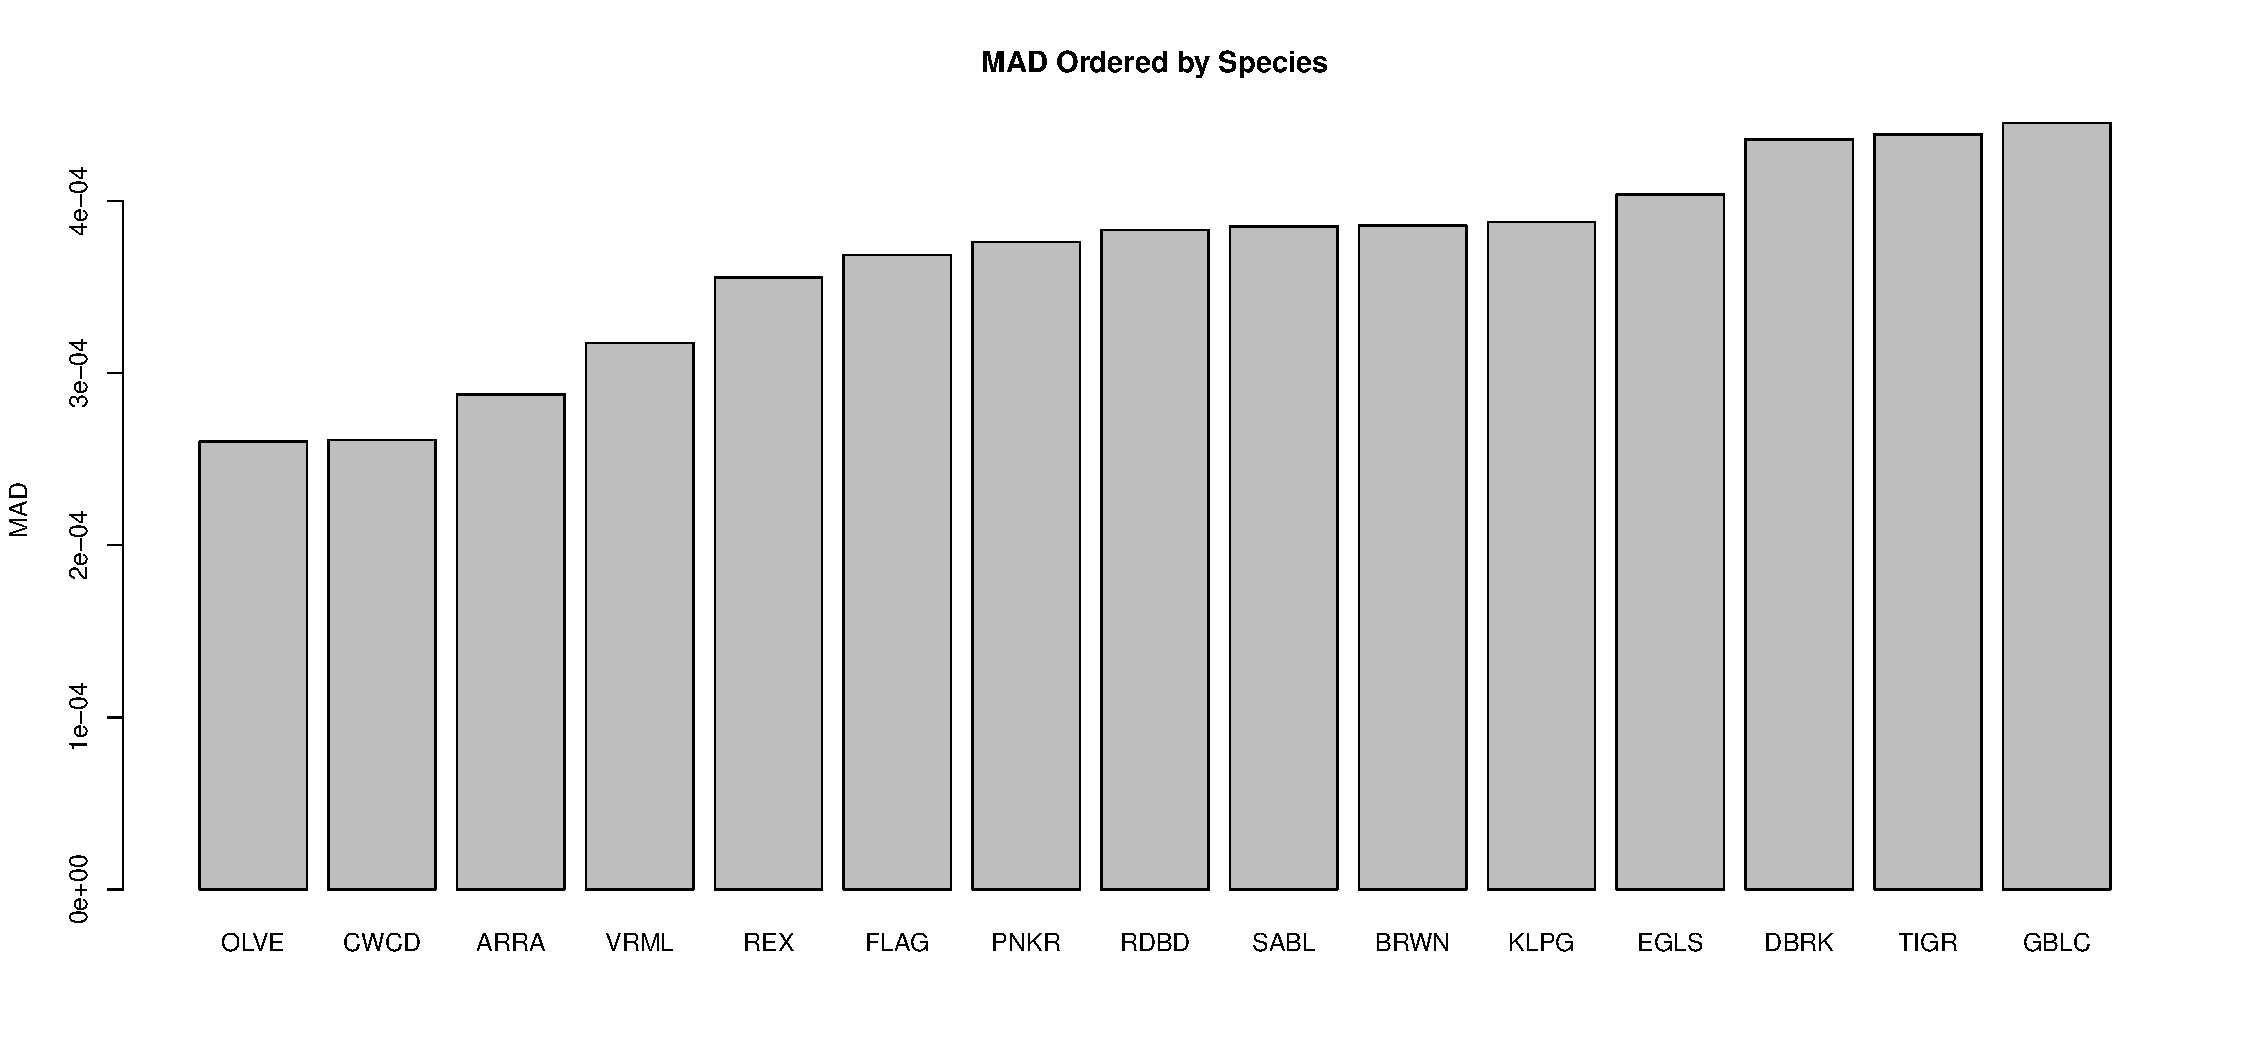
\includegraphics[width=0.6\textwidth]{../sscRuns/25319781982M4/sppMad68.pdf}
        \end{figure}

        \begin{figure}[ht!]
        \centering
        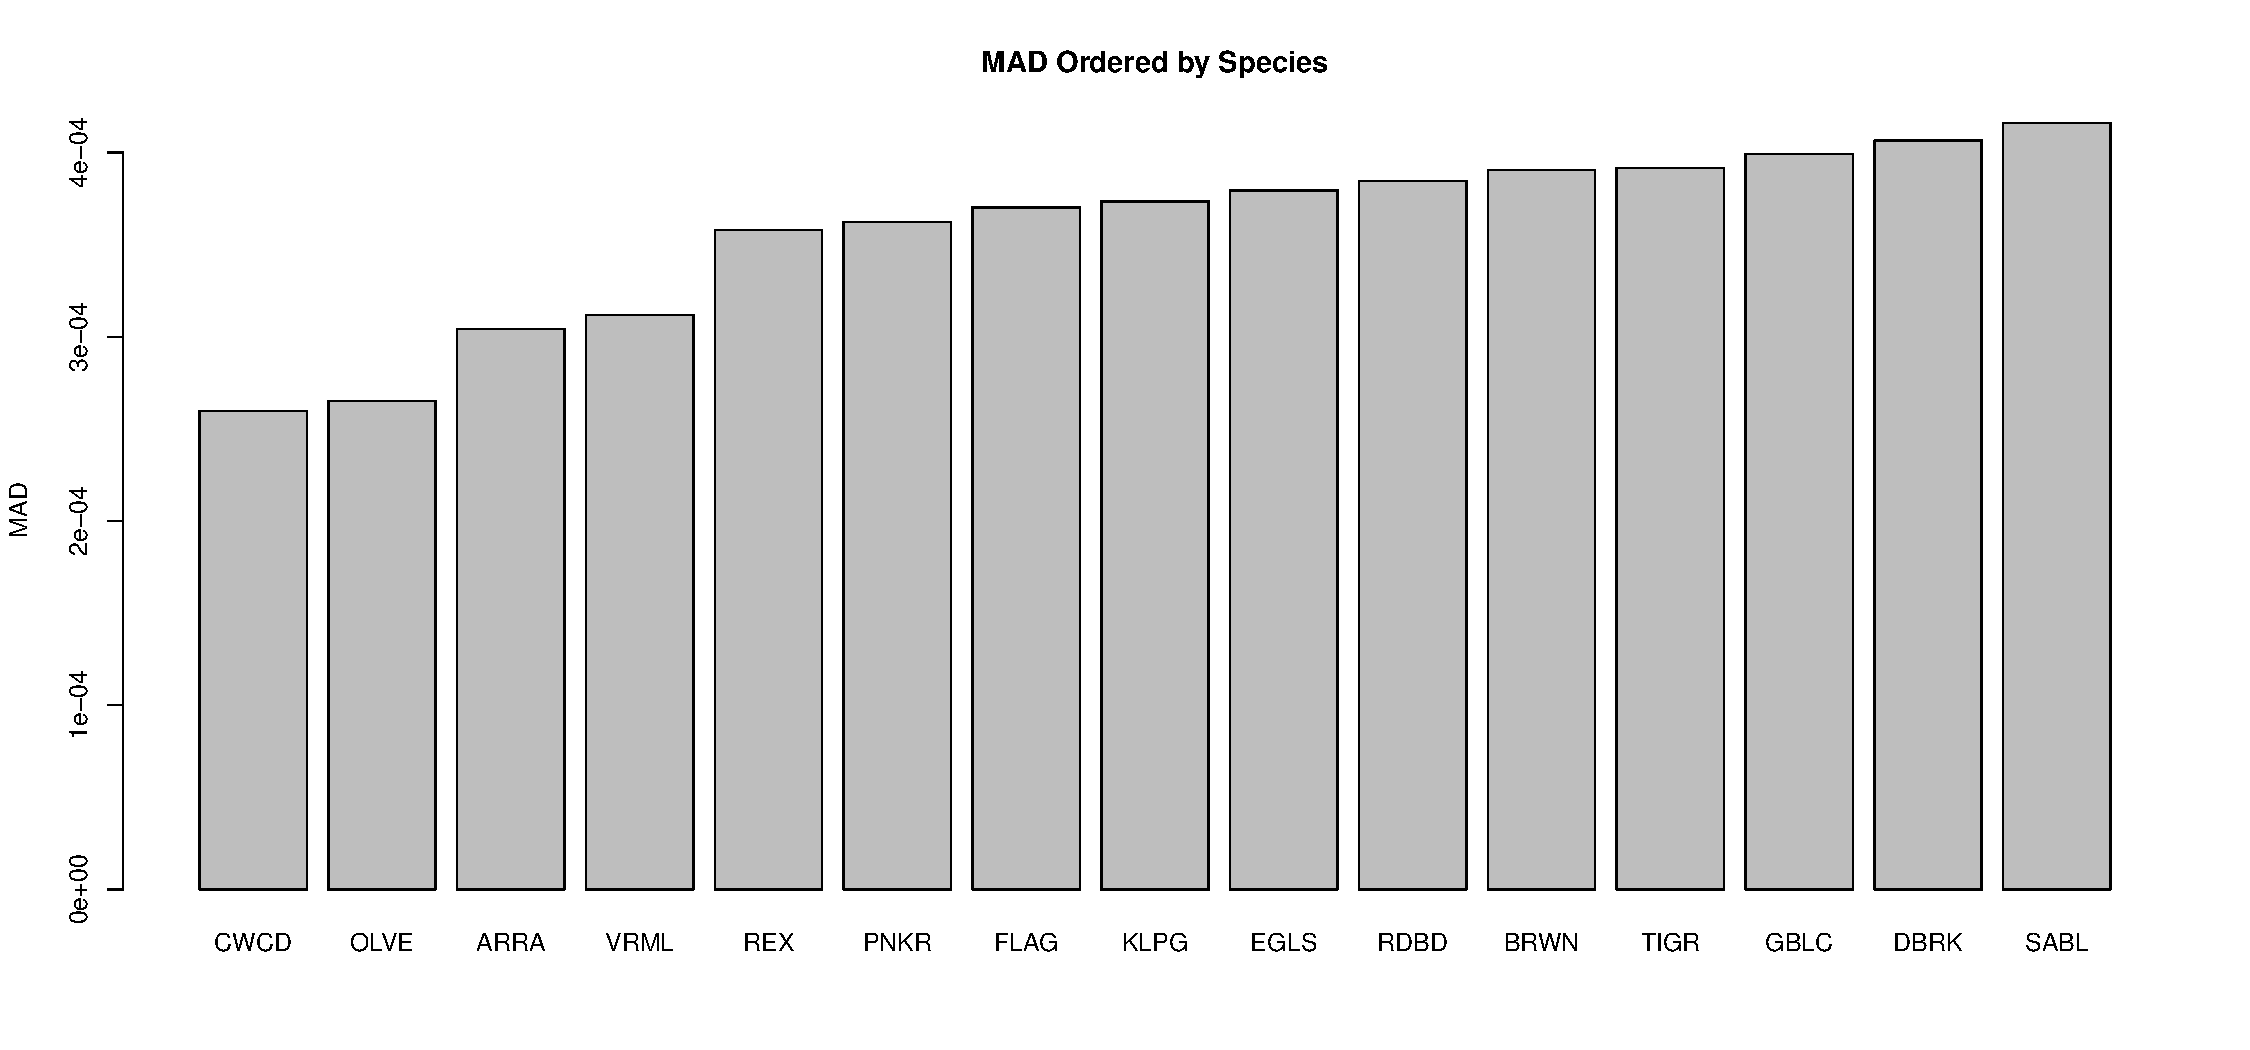
\includegraphics[width=0.6\textwidth]{../sscRuns/25319781982M5/sppMad68.pdf}
        \end{figure}

        \begin{figure}[ht!]
        \centering
        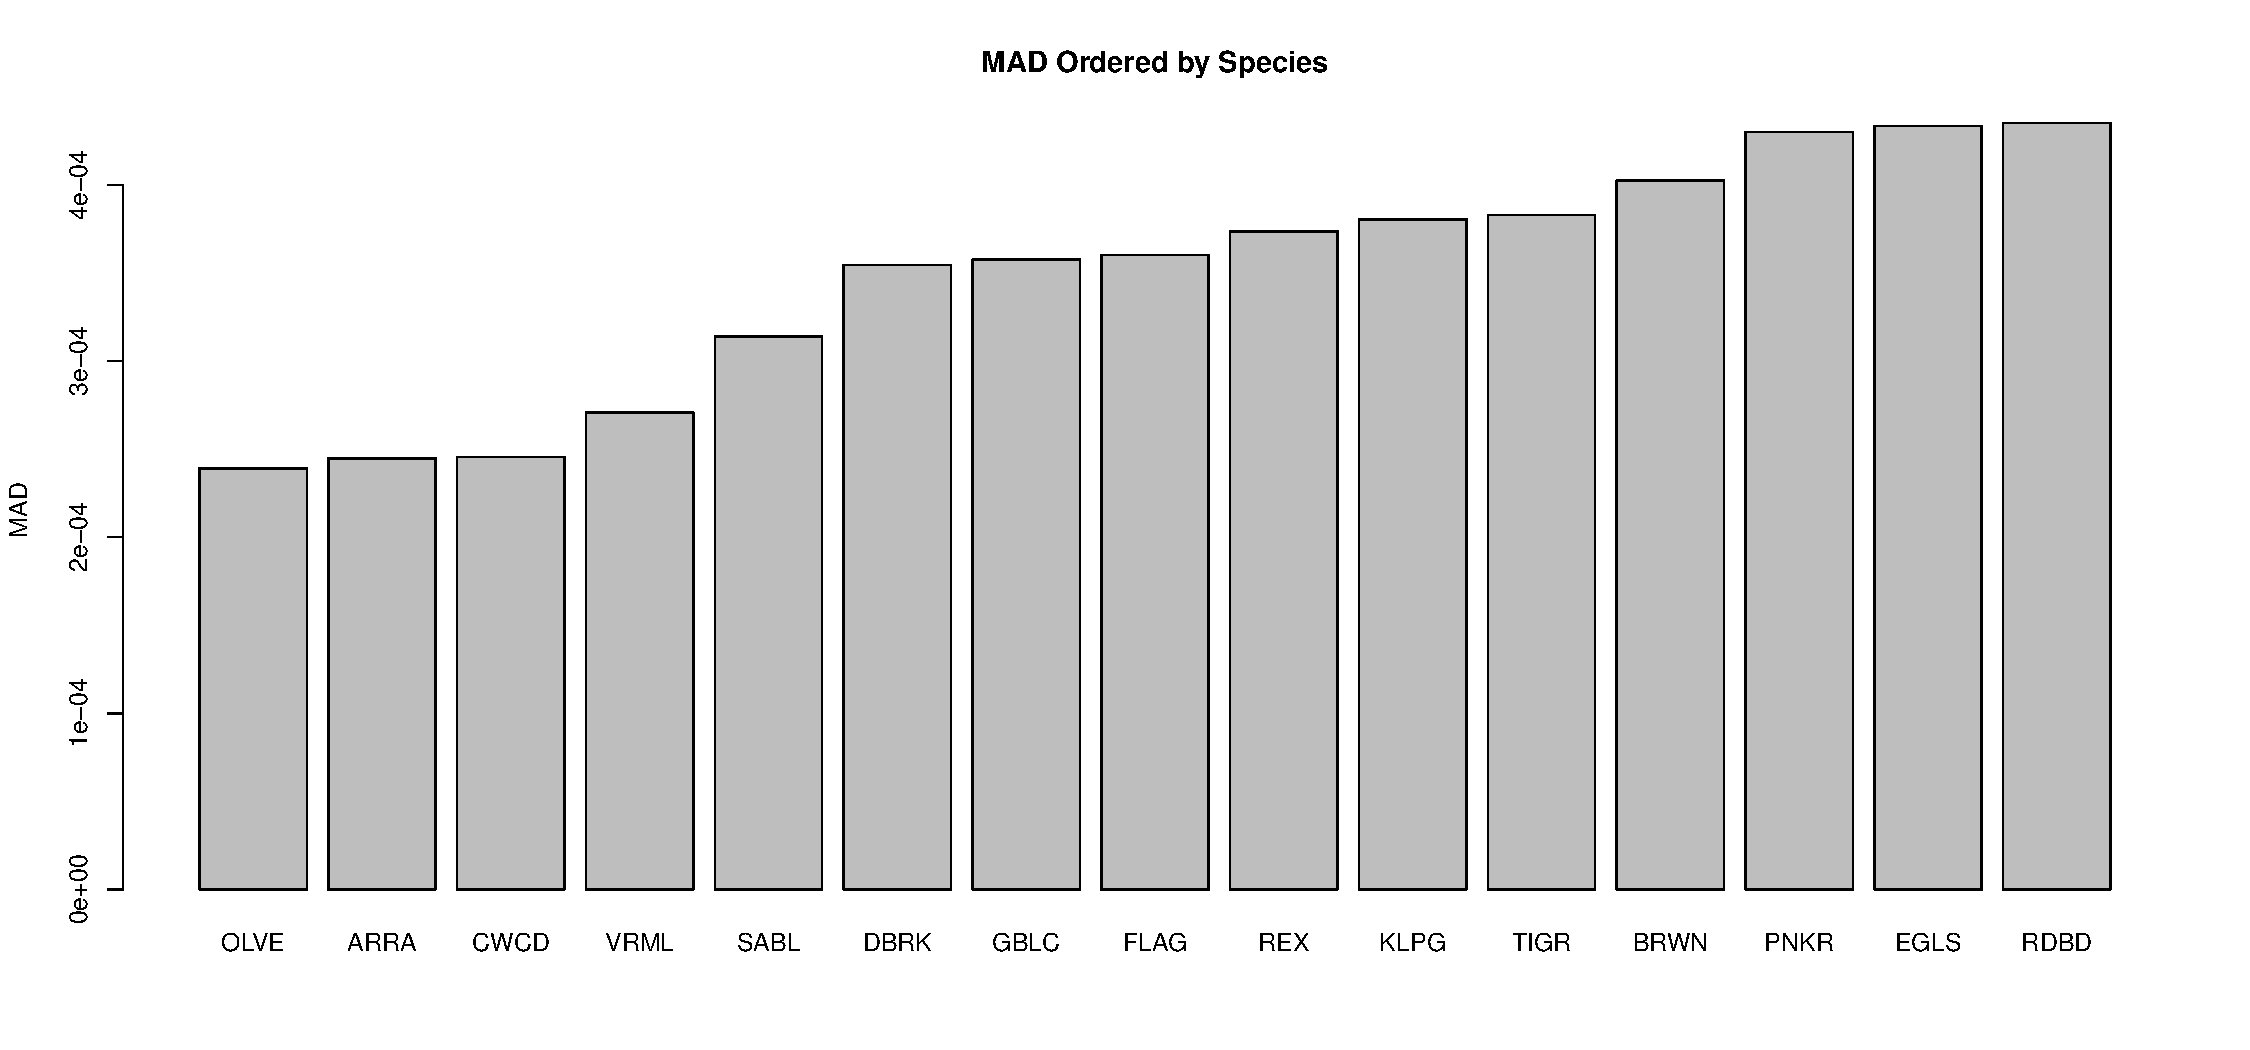
\includegraphics[width=0.6\textwidth]{../sscRuns/25319781982M6/sppMad68.pdf}
        \end{figure}

	\clearpage
        \begin{figure}[ht!]
        \centering
        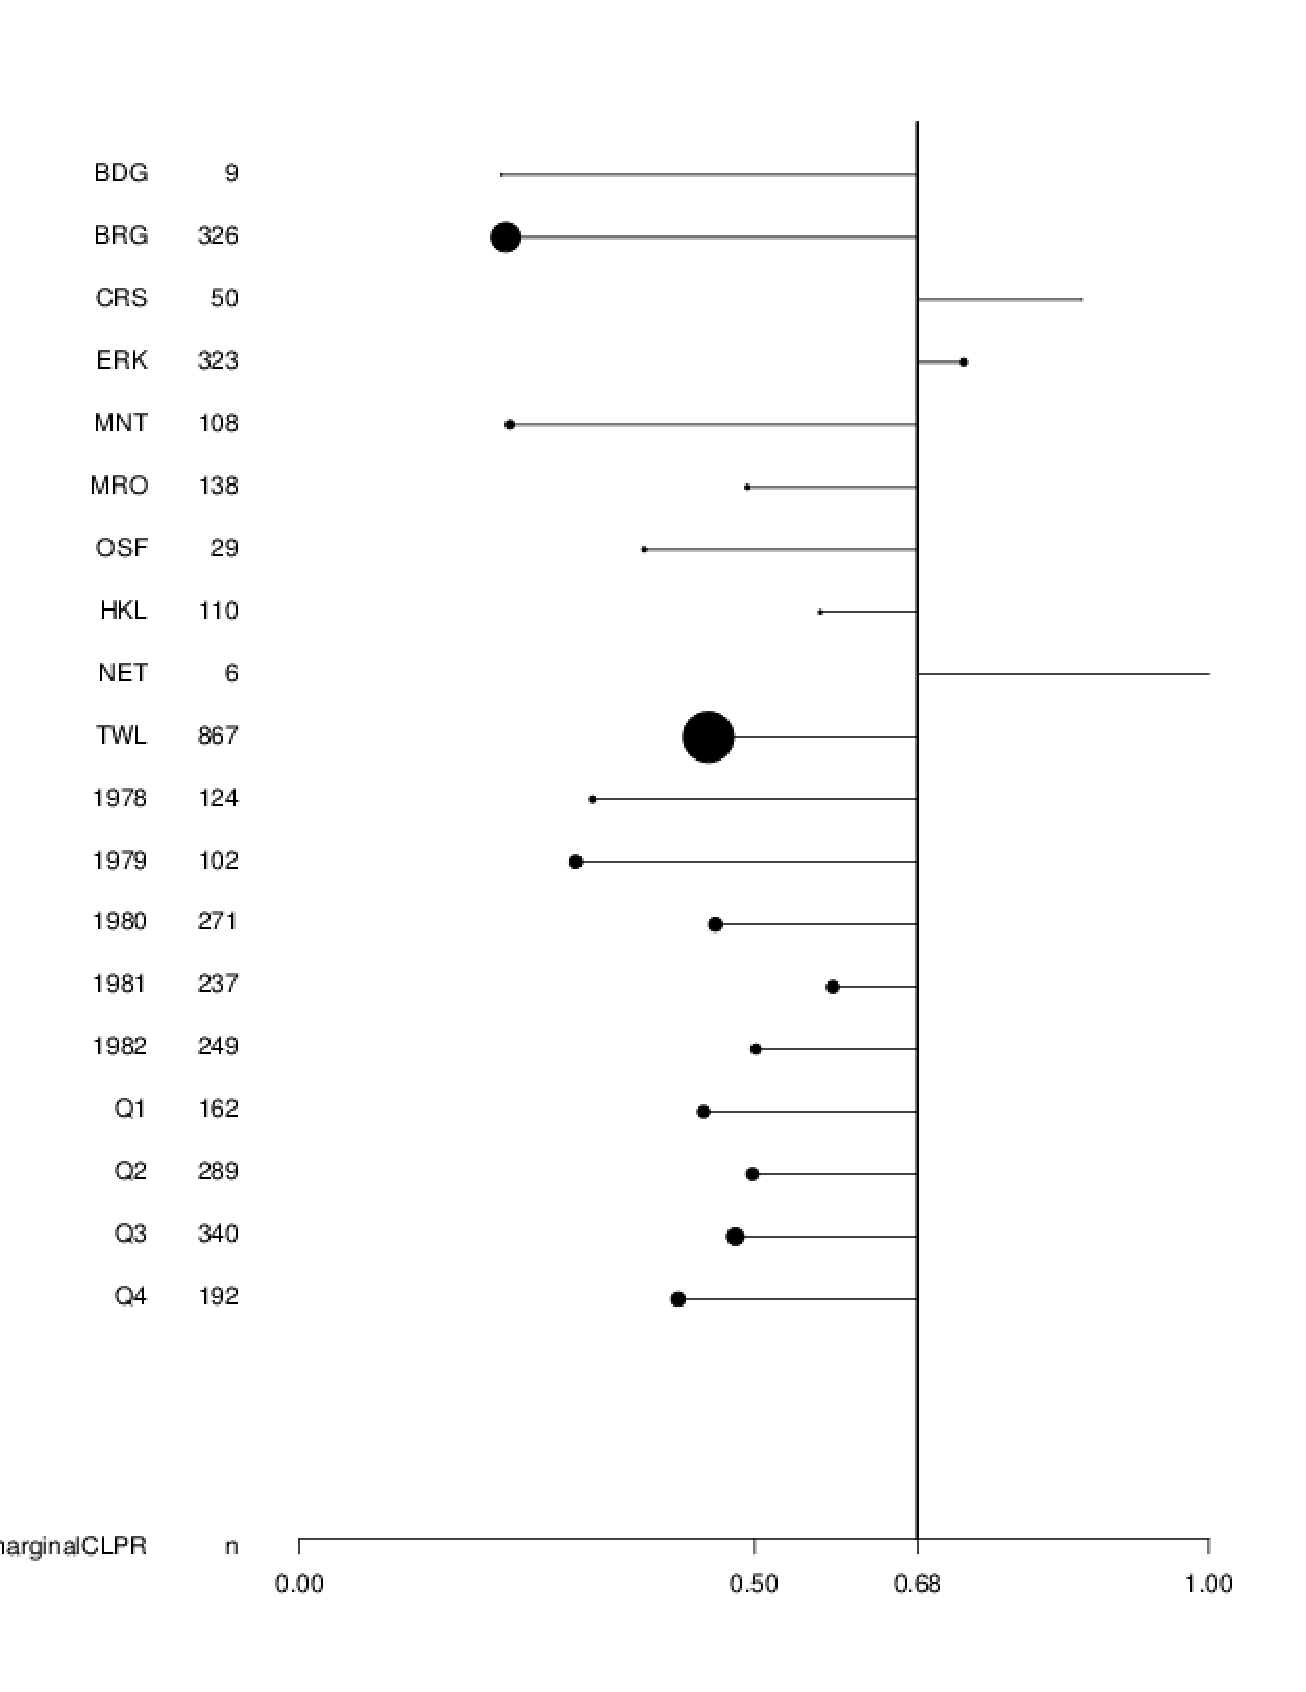
\includegraphics[width=1.1\textwidth]{{./postSSC/25319781982M4M5M6/marginalCLPR/marginalCLPR-0.68-Diagnostic}.pdf}
        \end{figure}

        \clearpage
        \begin{figure}[ht!]
        \centering
        \includegraphics[width=1.1\textwidth]{{./postSSC/25319781982M4M5M6/marginalWDOW/marginalWDOW-0.68-Diagnostic}.pdf}
        \end{figure}

        \clearpage
        \begin{figure}[ht!]
        \centering
        \includegraphics[width=1.1\textwidth]{{./postSSC/25319781982M4M5M6/marginalBRWN/marginalBRWN-0.68-Diagnostic}.pdf}
        \end{figure}

        \clearpage
        \begin{figure}[ht!]
        \centering
        \includegraphics[width=1.1\textwidth]{{./postSSC/25319781982M4M5M6/marginalDBRK/marginalDBRK-0.68-Diagnostic}.pdf}
        \end{figure}






%\subsubsection{M4}
%        \begin{figure}[ht!]
%        \centering
%        \includegraphics[width=1\textwidth]{../sscRuns/25319781982M4/sppMad68.pdf}
%        \end{figure}
%
%        \begin{figure}[ht!]
%        \centering
%        \includegraphics[width=1.1\textwidth]{{../sscRuns/25319781982M4/marginalCLPR/marginalCLPR-0.68-Diagnostic}.pdf}
%        \end{figure}
%
%        \begin{figure}[ht!]
%        \centering
%        \includegraphics[width=1.1\textwidth]{{../sscRuns/25319781982M4/marginalWDOW/marginalWDOW-0.68-Diagnostic}.pdf}
%        \end{figure} 
%        
%        \begin{figure}[ht!]
%        \centering
%        \includegraphics[width=1.1\textwidth]{{../sscRuns/25319781982M4/marginalOLVE/marginalOLVE-0.68-Diagnostic}.pdf}
%        \end{figure}
%
%        \begin{figure}[ht!]
%        \centering
%        \includegraphics[width=1.1\textwidth]{{../sscRuns/25319781982M4/marginalGBLC/marginalGBLC-0.68-Diagnostic}.pdf}
%        \end{figure}
%
%\clearpage
%\subsubsection{M5}
%	\begin{figure}[ht!]
%	\centering
%	\includegraphics[width=1\textwidth]{../sscRuns/25319781982M5/sppMad68.pdf}
%	\end{figure}
%
%	\begin{figure}[ht!]
%	\centering
%	\includegraphics[width=1.1\textwidth]{{../sscRuns/25319781982M5/marginalCLPR/marginalCLPR-0.68-Diagnostic}.pdf}
%	\end{figure}
%
%	\begin{figure}[ht!]
%	\centering
%	\includegraphics[width=1.1\textwidth]{{../sscRuns/25319781982M5/marginalWDOW/marginalWDOW-0.68-Diagnostic}.pdf}
%	\end{figure}
%	
%	\begin{figure}[ht!]
%	\centering
%	\includegraphics[width=1.1\textwidth]{{../sscRuns/25319781982M5/marginalCWCD/marginalCWCD-0.68-Diagnostic}.pdf}
%	\end{figure}
%
%	\begin{figure}[ht!]
%	\centering
%	\includegraphics[width=1.1\textwidth]{{../sscRuns/25319781982M5/marginalSABL/marginalSABL-0.68-Diagnostic}.pdf}
%	\end{figure}
%
%\clearpage
%\subsubsection{M6}
%	\begin{figure}[ht!]
%	\centering
%	\includegraphics[width=1\textwidth]{../sscRuns/25319781982M6/sppMad68.pdf}
%	\end{figure}
%
%	\begin{figure}[ht!]
%	\centering
%	\includegraphics[width=1.1\textwidth]{{../sscRuns/25319781982M6/marginalCLPR/marginalCLPR-0.68-Diagnostic}.pdf}
%	\end{figure}
%
%	\begin{figure}[ht!]
%	\centering
%	\includegraphics[width=1.1\textwidth]{{../sscRuns/25319781982M6/marginalWDOW/marginalWDOW-0.68-Diagnostic}.pdf}
%	\end{figure}
%	
%	\begin{figure}[ht!]
%	\centering
%	\includegraphics[width=1.1\textwidth]{{../sscRuns/25319781982M6/marginalOLVE/marginalOLVE-0.68-Diagnostic}.pdf}
%	\end{figure}
%
%	\begin{figure}[ht!]
%	\centering
%	\includegraphics[width=1.1\textwidth]{{../sscRuns/25319781982M6/marginalRDBD/marginalRDBD-0.68-Diagnostic}.pdf}
%	\end{figure}
%
\clearpage
\subsection{MCAT 253 Priors}
	\begin{table}[ht!]
        \centering
        \begin{tabular}[c]{@{}lcccccc@{}}
        %\toprule
        \hline
        & M4HC1 & M4HC3 & M4U4 \\ \hline
	\(\Delta\) DIC & 0.8 & 0.8 & 0 \\                                                 
	\(\Delta\) WAIC & 0.83 & 0.83 & 0 \\                                              
	\(pr(M|y)\) & 1 & 0 & 0
        \end{tabular}
        \end{table}

\subsubsection{\href{https://github.com/gasduster99/sppComp/tree/master/sscRuns/25319781982M4HC1}{M4HC1}, \href{https://github.com/gasduster99/sppComp/tree/master/sscRuns/25319781982M4HC3}{M4HC3}, \href{https://github.com/gasduster99/sppComp/tree/master/sscRuns/25319781982M4U4}{M4U4} \href{https://github.com/gasduster99/sppComp/tree/master/try1/postSSC/25319781982M4HC1HC3U4}{Comparision}}
	\begin{figure}[ht!]
	\centering
	\includegraphics[width=0.6\textwidth]{../sscRuns/25319781982M4HC1/sppMad68.pdf}
	\end{figure}
	
	\begin{figure}[ht!]
        \centering
        \includegraphics[width=0.6\textwidth]{../sscRuns/25319781982M4HC3/sppMad68.pdf}
        \end{figure}

	\begin{figure}[ht!]
        \centering
        \includegraphics[width=0.6\textwidth]{../sscRuns/25319781982M4U4/sppMad68.pdf}
        \end{figure}

	\clearpage
        \begin{figure}[ht!]
        \centering
        \includegraphics[width=1.1\textwidth]{{./postSSC/25319781982M4HC1HC3U4/marginalCLPR/marginalCLPR-0.68-Diagnostic}.pdf}
        \end{figure}

        \clearpage
        \begin{figure}[ht!]
        \centering
        \includegraphics[width=1.1\textwidth]{{./postSSC/25319781982M4HC1HC3U4/marginalWDOW/marginalWDOW-0.68-Diagnostic}.pdf}
        \end{figure}

        \clearpage
        \begin{figure}[ht!]
        \centering
        \includegraphics[width=1.1\textwidth]{{./postSSC/25319781982M4HC1HC3U4/marginalBRWN/marginalBRWN-0.68-Diagnostic}.pdf}
        \end{figure}

        \clearpage
        \begin{figure}[ht!]
        \centering
        \includegraphics[width=1.1\textwidth]{{./postSSC/25319781982M4HC1HC3U4/marginalDBRK/marginalDBRK-0.68-Diagnostic}.pdf}
        \end{figure}


%\subsubsection{M4HC1}
%	%\begin{figure}[ht!]
%	%\centering
%	%\includegraphics[width=1\textwidth]{../sscRuns/25019781982M4HC1/sppMad68.pdf}
%	%\end{figure}
%
%	\begin{figure}[ht!]
%	\centering
%	\includegraphics[width=0.8\textwidth]{{../sscRuns/25319781982M4HC1/marginalCLPR/marginalCLPR-0.68-Diagnostic}.pdf}
%	\end{figure}
%
%	\begin{figure}[ht!]
%	\centering
%	\includegraphics[width=1.1\textwidth]{{../sscRuns/25319781982M4HC1/marginalWDOW/marginalWDOW-0.68-Diagnostic}.pdf}
%	\end{figure}
%	
%	\begin{figure}[ht!]
%	\centering
%	\includegraphics[width=1.1\textwidth]{{../sscRuns/25319781982M4HC1/marginalOLVE/marginalOLVE-0.68-Diagnostic}.pdf}
%	\end{figure}
%
%	\begin{figure}[ht!]
%	\centering
%	\includegraphics[width=1.1\textwidth]{{../sscRuns/25319781982M4HC1/marginalGBLC/marginalGBLC-0.68-Diagnostic}.pdf}
%	\end{figure}
%
%\clearpage
%\subsubsection{M4HC3}
%	%\begin{figure}[ht!]
%	%\centering
%	%\includegraphics[width=1\textwidth]{../sscRuns/25019781982M4HC3/sppMad68.pdf}
%	%\end{figure}
%
%	\begin{figure}[ht!]
%	\centering
%	\includegraphics[width=0.9\textwidth]{{../sscRuns/25319781982M4HC3/marginalCLPR/marginalCLPR-0.68-Diagnostic}.pdf}
%	\end{figure}
%
%	\begin{figure}[ht!]
%	\centering
%	\includegraphics[width=1.1\textwidth]{{../sscRuns/25319781982M4HC3/marginalWDOW/marginalWDOW-0.68-Diagnostic}.pdf}
%	\end{figure}
%	
%	\begin{figure}[ht!]
%	\centering
%	\includegraphics[width=1.1\textwidth]{{../sscRuns/25319781982M4HC3/marginalOLVE/marginalOLVE-0.68-Diagnostic}.pdf}
%	\end{figure}
%
%	\begin{figure}[ht!]
%	\centering
%	\includegraphics[width=1.1\textwidth]{{../sscRuns/25319781982M4HC3/marginalGBLC/marginalGBLC-0.68-Diagnostic}.pdf}
%	\end{figure}	
%
%\clearpage
%\subsubsection{M4U4}
%	%\begin{figure}[ht!]
%	%\centering
%	%\includegraphics[width=1\textwidth]{../sscRuns/25019781982M4U4/sppMad68.pdf}
%	%\end{figure}
%
%	\begin{figure}[ht!]
%	\centering
%	\includegraphics[width=0.9\textwidth]{{../sscRuns/25319781982M4U4/marginalCLPR/marginalCLPR-0.68-Diagnostic}.pdf}
%	\end{figure}
%
%	\begin{figure}[ht!]
%	\centering
%	\includegraphics[width=1.1\textwidth]{{../sscRuns/25319781982M4U4/marginalWDOW/marginalWDOW-0.68-Diagnostic}.pdf}
%	\end{figure}
%	
%	\begin{figure}[ht!]
%	\centering
%	\includegraphics[width=1.1\textwidth]{{../sscRuns/25319781982M4U4/marginalOLVE/marginalOLVE-0.68-Diagnostic}.pdf}
%	\end{figure}
%
%	\begin{figure}[ht!]
%	\centering
%	\includegraphics[width=1.1\textwidth]{{../sscRuns/25319781982M4U4/marginalGBLC/marginalGBLC-0.68-Diagnostic}.pdf}
%	\end{figure}	

\clearpage
\subsection{MCAT 269 Time Models}
	\begin{table}[h!]
	\centering
	\begin{tabular}[c]{@{}lcccccc@{}}
	%\toprule
	\hline
	& M1 & M2 & M3 & M4 & M5 & M6 \\ \hline
	\(\Delta\) DIC & 572.51 & 176.63 & 599.41 & 0.57 & 0 & 193.35 \\
	\(\Delta\) WAIC & 427.48 & 69.37 & 454.41 & 0.23 & 0 & 78.07 \\
	\(pr(M|y)\) & 0 & 0 & 0 & 0 & 0 & 1	
	\end{tabular}
	\end{table}
	
\subsubsection{\href{https://github.com/gasduster99/sppComp/tree/master/sscRuns/26919781982M4}{M4}, \href{https://github.com/gasduster99/sppComp/tree/master/sscRuns/26919781982M5}{M5}, \href{https://github.com/gasduster99/sppComp/tree/master/sscRuns/26919781982M6}{M6} \href{https://github.com/gasduster99/sppComp/tree/master/try1/postSSC/26919781982M4M5M6}{Comparision}}
        \begin{figure}[ht!]
        \centering
        \includegraphics[width=0.6\textwidth]{../sscRuns/26919781982M4/sppMad68.pdf}
        \end{figure}

	\begin{figure}[ht!]
        \centering
        \includegraphics[width=0.6\textwidth]{../sscRuns/26919781982M5/sppMad68.pdf}
        \end{figure}
	
	\begin{figure}[ht!]
        \centering
        \includegraphics[width=0.6\textwidth]{../sscRuns/26919781982M6/sppMad68.pdf}
        \end{figure}

	\clearpage
        \begin{figure}[ht!]
        \centering
        \includegraphics[width=1.1\textwidth]{{./postSSC/26919781982M4M5M6/marginalYTRK/marginalYTRK-0.68-Diagnostic}.pdf}
        \end{figure}

	\clearpage
        \begin{figure}[ht!]
        \centering
        \includegraphics[width=1.1\textwidth]{{./postSSC/26919781982M4M5M6/marginalCLPR/marginalCLPR-0.68-Diagnostic}.pdf}
        \end{figure}

        \clearpage
        \begin{figure}[ht!]
        \centering
        \includegraphics[width=1.1\textwidth]{{./postSSC/26919781982M4M5M6/marginalBCAC/marginalBCAC-0.68-Diagnostic}.pdf}
        \end{figure}

        \clearpage
        \begin{figure}[ht!]
        \centering
        \includegraphics[width=1.1\textwidth]{{./postSSC/26919781982M4M5M6/marginalWDOW/marginalWDOW-0.68-Diagnostic}.pdf}
        \end{figure}
 

%	\begin{figure}[ht!]
%        \centering
%        \includegraphics[width=1.1\textwidth]{{../sscRuns/26919781982M4/marginalYTRK/marginalYTRK-0.68-Diagnostic}.pdf}
%        \end{figure}
%	
%        \begin{figure}[ht!]
%        \centering
%        \includegraphics[width=1.1\textwidth]{{../sscRuns/26919781982M4/marginalCLPR/marginalCLPR-0.68-Diagnostic}.pdf}
%        \end{figure}
%
%        \begin{figure}[ht!]
%        \centering
%        \includegraphics[width=1.1\textwidth]{{../sscRuns/26919781982M4/marginalBCAC/marginalBCAC-0.68-Diagnostic}.pdf}
%        \end{figure}  
%
%        \begin{figure}[ht!]
%        \centering
%        \includegraphics[width=1.1\textwidth]{{../sscRuns/26919781982M4/marginalWDOW/marginalWDOW-0.68-Diagnostic}.pdf}
%        \end{figure}
%
%\clearpage
%\subsubsection{M5}
%        \begin{figure}[ht!]
%        \centering
%        \includegraphics[width=1\textwidth]{../sscRuns/25319781982M5/sppMad68.pdf}
%        \end{figure}
%
%	\begin{figure}[ht!]
%        \centering
%        \includegraphics[width=1.1\textwidth]{{../sscRuns/26919781982M5/marginalYTRK/marginalYTRK-0.68-Diagnostic}.pdf}
%        \end{figure}
%	
%        \begin{figure}[ht!]
%        \centering
%        \includegraphics[width=1.1\textwidth]{{../sscRuns/26919781982M5/marginalCLPR/marginalCLPR-0.68-Diagnostic}.pdf}
%        \end{figure}
%
%        \begin{figure}[ht!]
%        \centering
%        \includegraphics[width=1.1\textwidth]{{../sscRuns/26919781982M5/marginalBCAC/marginalBCAC-0.68-Diagnostic}.pdf}
%        \end{figure}  
%
%        \begin{figure}[ht!]
%        \centering
%        \includegraphics[width=1.1\textwidth]{{../sscRuns/26919781982M5/marginalWDOW/marginalWDOW-0.68-Diagnostic}.pdf}
%        \end{figure}
%
%\clearpage
%\subsubsection{M6}
%        \begin{figure}[ht!]
%        \centering
%        \includegraphics[width=1\textwidth]{../sscRuns/25319781982M6/sppMad68.pdf}
%        \end{figure}
%
%	\begin{figure}[ht!]
%        \centering
%        \includegraphics[width=1.1\textwidth]{{../sscRuns/26919781982M6/marginalYTRK/marginalYTRK-0.68-Diagnostic}.pdf}
%        \end{figure}
%	
%        \begin{figure}[ht!]
%        \centering
%        \includegraphics[width=1.1\textwidth]{{../sscRuns/26919781982M6/marginalCLPR/marginalCLPR-0.68-Diagnostic}.pdf}
%        \end{figure}
%
%        \begin{figure}[ht!]
%        \centering
%        \includegraphics[width=1.1\textwidth]{{../sscRuns/26919781982M6/marginalBCAC/marginalBCAC-0.68-Diagnostic}.pdf}
%        \end{figure}  
%
%        \begin{figure}[ht!]
%        \centering
%        \includegraphics[width=1.1\textwidth]{{../sscRuns/26919781982M6/marginalWDOW/marginalWDOW-0.68-Diagnostic}.pdf}
%        \end{figure}

\clearpage
\subsection{MCAT 269 Priors}
	\begin{table}[ht!]
        \centering
        \begin{tabular}[c]{@{}lcccccc@{}}
        %\toprule
        \hline
        & M4HC1 & M4HC3 & M4U4 \\ \hline
	\(\Delta\) DIC & 176.33 & 0.2 & 0 \\                                              
	\(\Delta\) WAIC & 69.19 & 0.08 & 0 \\                                             
	\(pr(M|y)\) & 1 & 0 & 0
        \end{tabular}
        \end{table}

\subsubsection{\href{https://github.com/gasduster99/sppComp/tree/master/sscRuns/26919781982M4HC1}{M4HC1}, \href{https://github.com/gasduster99/sppComp/tree/master/sscRuns/26919781982M4HC3}{M4HC3}, \href{https://github.com/gasduster99/sppComp/tree/master/sscRuns/26919781982M4U4}{M4U4} \href{https://github.com/gasduster99/sppComp/tree/master/try1/postSSC/26919781982M4HC1HC3U4}{Comparision}}
        \begin{figure}[ht!]
        \centering
        \includegraphics[width=0.6\textwidth]{../sscRuns/26919781982M4HC1/sppMad68.pdf}
        \end{figure}

        \begin{figure}[ht!]
        \centering
        \includegraphics[width=0.6\textwidth]{../sscRuns/26919781982M4HC3/sppMad68.pdf}
        \end{figure}

        \begin{figure}[ht!]
        \centering
        \includegraphics[width=0.6\textwidth]{../sscRuns/26919781982M4U4/sppMad68.pdf}
	\end{figure}

        \clearpage
        \begin{figure}[ht!]
        \centering
        \includegraphics[width=1.1\textwidth]{{./postSSC/26919781982M4HC1HC3U4/marginalYTRK/marginalYTRK-0.68-Diagnostic}.pdf}
        \end{figure}

        \clearpage
        \begin{figure}[ht!]
        \centering
        \includegraphics[width=1.1\textwidth]{{./postSSC/26919781982M4HC1HC3U4/marginalCLPR/marginalCLPR-0.68-Diagnostic}.pdf}
        \end{figure}

        \clearpage
        \begin{figure}[ht!]
        \centering
        \includegraphics[width=1.1\textwidth]{{./postSSC/26919781982M4HC1HC3U4/marginalBCAC/marginalBCAC-0.68-Diagnostic}.pdf}
        \end{figure}

        \clearpage
        \begin{figure}[ht!]
        \centering
        \includegraphics[width=1.1\textwidth]{{./postSSC/26919781982M4HC1HC3U4/marginalWDOW/marginalWDOW-0.68-Diagnostic}.pdf}
        \end{figure}

	

%\subsubsection{M4HC1}
%        %\begin{figure}[ht!]
%        %\centering
%        %\includegraphics[width=1\textwidth]{../sscRuns/25019781982M4HC1/sppMad68.pdf}
%        %\end{figure}
%
%        \begin{figure}[ht!]
%        \centering
%        \includegraphics[width=0.8\textwidth]{{../sscRuns/26919781982M4HC1/marginalYTRK/marginalYTRK-0.68-Diagnostic}.pdf}
%        \end{figure}
%
%        \begin{figure}[ht!]
%        \centering
%        \includegraphics[width=1.1\textwidth]{{../sscRuns/26919781982M4HC1/marginalCLPR/marginalCLPR-0.68-Diagnostic}.pdf}
%        \end{figure}
%
%        \begin{figure}[ht!]
%        \centering
%        \includegraphics[width=1.1\textwidth]{{../sscRuns/26919781982M4HC1/marginalBCAC/marginalBCAC-0.68-Diagnostic}.pdf}
%        \end{figure}
%
%        \begin{figure}[ht!]
%        \centering
%        \includegraphics[width=1.1\textwidth]{{../sscRuns/26919781982M4HC1/marginalWDOW/marginalWDOW-0.68-Diagnostic}.pdf}
%        \end{figure}
%
%\clearpage
%\subsubsection{M4HC3}
%        %\begin{figure}[ht!]
%        %\centering
%        %\includegraphics[width=1\textwidth]{../sscRuns/25019781982M4HC1/sppMad68.pdf}
%        %\end{figure}
%
%        \begin{figure}[ht!]
%        \centering
%        \includegraphics[width=0.9\textwidth]{{../sscRuns/26919781982M4HC3/marginalYTRK/marginalYTRK-0.68-Diagnostic}.pdf}
%        \end{figure}
%
%        \begin{figure}[ht!]
%        \centering
%        \includegraphics[width=1.1\textwidth]{{../sscRuns/26919781982M4HC3/marginalCLPR/marginalCLPR-0.68-Diagnostic}.pdf}
%        \end{figure}
%
%        \begin{figure}[ht!]
%        \centering
%        \includegraphics[width=1.1\textwidth]{{../sscRuns/26919781982M4HC3/marginalBCAC/marginalBCAC-0.68-Diagnostic}.pdf}
%        \end{figure}
%
%        \begin{figure}[ht!]
%        \centering
%        \includegraphics[width=1.1\textwidth]{{../sscRuns/26919781982M4HC3/marginalWDOW/marginalWDOW-0.68-Diagnostic}.pdf}
%        \end{figure}
%
%\clearpage
%\subsubsection{M4U4}
%        %\begin{figure}[ht!]
%        %\centering
%        %\includegraphics[width=1\textwidth]{../sscRuns/25019781982M4HC1/sppMad68.pdf}
%        %\end{figure}
%
%        \begin{figure}[ht!]
%        \centering
%        \includegraphics[width=0.9\textwidth]{{../sscRuns/26919781982M4U4/marginalYTRK/marginalYTRK-0.68-Diagnostic}.pdf}
%        \end{figure}
%
%        \begin{figure}[ht!]
%        \centering
%        \includegraphics[width=1.1\textwidth]{{../sscRuns/26919781982M4U4/marginalCLPR/marginalCLPR-0.68-Diagnostic}.pdf}
%        \end{figure}
%
%        \begin{figure}[ht!]
%        \centering
%        \includegraphics[width=1.1\textwidth]{{../sscRuns/26919781982M4U4/marginalBCAC/marginalBCAC-0.68-Diagnostic}.pdf}
%        \end{figure}
%
%        \begin{figure}[ht!]
%        \centering
%        \includegraphics[width=1.1\textwidth]{{../sscRuns/26919781982M4U4/marginalWDOW/marginalWDOW-0.68-Diagnostic}.pdf}
%        \end{figure}

%\clearpage
%\subsubsection{M4}
%        \begin{figure}[ht!]
%        \centering
%        \includegraphics[width=1\textwidth]{../sscRuns/26919781982M4/sppMad68.pdf}
%        \end{figure}
%
%	\begin{figure}[ht!]
%        \centering
%        \includegraphics[width=1.1\textwidth]{{../sscRuns/26919781982M4/marginalYTRK/marginalYTRK-0.68-Diagnostic}.pdf}
%        \end{figure}
%	
%        \begin{figure}[ht!]
%        \centering
%        \includegraphics[width=1.1\textwidth]{{../sscRuns/26919781982M4/marginalCLPR/marginalCLPR-0.68-Diagnostic}.pdf}
%        \end{figure}
%
%        \begin{figure}[ht!]
%        \centering
%        \includegraphics[width=1.1\textwidth]{{../sscRuns/26919781982M4/marginalBCAC/marginalBCAC-0.68-Diagnostic}.pdf}
%        \end{figure}  
%
%        \begin{figure}[ht!]
%        \centering
%        \includegraphics[width=1.1\textwidth]{{../sscRuns/26919781982M4/marginalWDOW/marginalWDOW-0.68-Diagnostic}.pdf}
%        \end{figure}


%%
%\clearpage
%%
%\section{Diagnostic sensitivity to alternative time-blocking}
%
%%
%\clearpage
%%
%\section{Species:Port and Species:Gear interactions}
%
%%
%\clearpage
%%
%\section{Landings Comparision}
%
%%
%\clearpage
%%
%\section{Time block species sample sizes}
%
%%
%\clearpage
%%
%\section{Model mispecification self-test}













%%
%\clearpage
%%
%\section{Diagnostic template and fully stratified predictive performance}





\end{document}
